%% \documentclass{aastex}
\documentclass{emulateapj}

\usepackage{graphicx}
\usepackage{verbatim}
\usepackage{booktabs} % For toprule and bottomrule in tables
\usepackage{multirow}
\usepackage{amsmath}


\newcommand{\pasa}{PASA}               % PASA

\shorttitle{To be decided by committee after the Summer Solstice}
\shortauthors{Casey, Keller and Da Costa}

\begin{document}

	\title{To be decided by committee after the Solstice}
	\author{Andy Casey, Stefan Keller, Gary Da Costa}
	\affil{	Research School of Astronomy \& Astrophysics,
		Australian National University,
		Canberra, Australia}
		
	
	\begin{abstract}

	\end{abstract}
	
	\keywords{Galaxy: halo, structure --- Stars: abundances}
	
	
	
	
	\section{Introduction}
	
	The proportion of substructure uncovered in the Galactic stellar halo over the last few decades has highlighted the crucial involvement accretion has played in the formation of the Milky Way. Properties of these stellar structures allow us to probe both the formation mechanisms and history of the Galaxy. This technique of studying stellar populations as surrogates of galactic archeology was first proposed in the seminal paper of \citet{Eggen;Lynden-Bell;Sandage_1962} who observed a metallicity abundance declivity in stars from the disk to the halo. From these measurements they inferred that  the Galaxy formed by a rapid collapse of a relatively homogenous protogalactic cloud. In contrast of this inference, \citet{Searle;Zinn_1978} observed a wide scope of metallicities within globular clusters irrespective of their galactocentric distance, which implied a formation paradigm based on the hierarchical accretion of protogalactic fragments. Recent studies \citep{Carollo;et-al_2007, Carollo;et-al_2010} have suggested multiple evolution mechanisms are required for galaxy formation to reconcile observational evidence, although this is a subject for ongoing debate. Regardless, the quiescent dissipation-less merging paradigm is widely accepted, and consistent with favoured Cold Dark Matter ($\Lambda$CDM) cosmology models. Through the examination of ongoing accretion events in the Milky Way and fossils from previous mergers, we can ultimately trace the formation history of the Galaxy. 
	
		
	The stellar halo has formed at least partly \citep{Starkenburg;et-al_2009}, if not entirely by accretion. \citet{Bell;et-al_2008} compared observations from the Sloan Digital Sky Survey \citep[hereafter SDSS]{York;et-al_2000} to simulations and found that observations are consistent with the stellar halo being entirely formed by the hierarchical merging of accreted satellites.
	
	
	Unquestionably the most prominent accretion event within the Milky Way is that of the Sagittarius (Sgr) dwarf Spheroidal (dSph) galaxy. Originally uncovered by \citet{Ibata;et-al_1994} as a co-moving group of K- and M-type giants, the tidal tails of Sgr circle our Galaxy, and as such they have been extensively traced with red-clump stars \citep{Majewski;et-al_1999}, carbon stars \citep{Totten;Irwin_1998, Ibata;et-al_2001}, RR Lyrae stars \citep{Ivezic;et-al_2000, Vivas;et-al_2005, Watkins;et-al_2009, Prior;et-al_2009a}, A-type stars \citep{Newberg;et-al_2003} and K/M-giants \citep{Majewski;et-al_2003}. With spatial and kinematical information, tracers originating from the dwarf progenitor can be unequivocally identified. This is because they remain dynamically cold and identifiable as kinematic substructure long after they are stripped from their progenitor \citep{Ibata;Lewis_1998, Helmi;White_1999}. 
	
	
	Stellar tracers within these tails are kinematically sensitive to the galactic potential. Their bulk kinematic signature is reflective of the shape and quantity of dark matter in the Milky Way. This has led various groups to model the Sgr tidal tails in different galactic potentials. \citet{Martinez-Delgado;et-al_2004} traced the northern arm and found a near spherical or oblate ($q \approx 0.85$) dark matter halo best represented the observed debris, which coincides with the findings of \citet{Ibata;et-al_2001}. In contrast, \citet{Helmi_2004} found evidence in the Sgr leading debris kinematics that most favoured a prolate ($q = 1.25$) halo. \citet{Vivas;et-al_2005} found that either the prolate or spherical models of  \citet{Helmi_2004} best fit their observed RR Lyrae data than those of an oblate model. \citet{Johnston;et-al_2005} later pointed out that no prolate model can reproduce the orbital pole procession of the Sgr debris, but an oblate potential excellently replicated the procession. \citet[hereafter LJM05]{Law;et-al_2005} performed simulations using data of the Sgr debris from the 2-Micron All Sky Survey (2MASS) catalogue and found that the kinematics of leading debris was best fit by prolate halos, whereas the trailing debris favoured oblate halos. 
	
	
	\citet{Belokurov;et-al_2006} found an apparent bifurcation within the Sgr debris, which \citet{Fellhauer;et-al_2006} argued can only result with by a dark halo having close to a spherical shape. \citet{Law;et-al_2009} introduced a tri-axial model with a varying flattenning profile $q$ which replicates the orbital procession seen, and kinematically matches observations of the Sgr debris. However, \citet{Law;Majewski_2010} (hereafter LM10) concedes this may be a purely numerical solution as tri-axial halos are dynamically unstable, and admits more kinematic observations in other regions of the Sgr stream are required.


	After the Sgr stellar stream, the Virgo Over-Density (VOD) is arguably the next most significant substructure within our Galaxy. The first over-density in the vicinity of the VOD was observed as a group of RR Lyrae stars ~13 kpc away by the QUEST survey \citep{Vivas;et-al_2001}. The collaboration later named this the ``$12\fh4$ clump'' \citep{Zinn;et-al_2004}. The broad nature of the VOD as a diffuse over-density of main-sequence turnoff stars centered at $r_\odot \sim18 \text{kpc}$ \citep[which ][dubbed as S297+63-20.5]{Newberg;et-al_2002} was uncovered within the SDSS catalogue. The nomenclature on the substructure names within this region is varied, however when referring to the VOD we are discussing the spatial over-density of stars within the region which includes numerous distinct superimposed moving groups. Within the VOD itself, multiple studies find a peak density of RR Lyrae \citep{Vivas;et-al_2001, Ivezic;et-al_2005} and F-type main sequence stars \citep{Newberg;et-al_2002} at (R.A., Dec) = (190$^\circ$, 0$^\circ$). Close by, \citet{Juric;et-al_2008} find the F-type main sequence peak at (R.A., Dec) = (192$^\circ$, +2$^\circ$) and \citet{Keller_2010} finds the sub-giant peak density at (R.A., Dec) = (194.6$^\circ$, +1.8$^\circ$). The exact spatial centroid of the VOD remains equivocal, and appears to be influenced by the selection effects of stellar type.	
	
	
	%, which was  found to be a co-moving group and was titled the Virgo Stellar Stream \citep[VSS;]{Duffau;et-al_2006} to distinguish it from the VOD.%
	
	Furthermore, the spatial bounds of the VOD remains unclear. There is some agreement that the boundaries of the structure extend outside the SDSS catalogue \citep{Newberg;et-al_2007,Prior;et-al_2009a,Keller;et-al_2009}. Observations to date represent lower limits on the VOD extent.\citet{Juric;et-al_2008} used photometric parallaxes to describe a diffuse over-density spanning $\sim$1000 deg$^2$, whereas \citet{Prior;et-al_2009a} estimated a coverage of $\sim$760 deg$^2$ from the luminosity function excess in the region. \citet{Duffau;et-al_2006} previously used a similar technique to \citet{Prior;et-al_2009a} and yielded a minimum sky coverage of 106 deg$^2$. A spatial boundary of 144 deg$^2$ was derived by \citet{Keller_2010} for the VOD from the luminosity function excess of sub-giants, which is more in-line with \citet{Duffau;et-al_2006} as a lower limit than other studies, which \citet{Keller_2010} attributes to low resolution data. 
	
	
	Within this region of sky there are multiple substructures along the line of sight. \citet{Duffau;et-al_2006} took observations of BHB and RR Lyrae within the ``$12\fh4$ clump'' and found a common velocity of $V_{GSR} = 99.8$ km s$^{-1}$ with $\sigma = 17.3$ km s$^{-1}$. This kinematic distinction from the VOD was strengthened by distance estimations which placed the VOD centroid at $r_{\odot} = 16 \text{kpc}$ \citep{Juric;et-al_2008, Keller_2010}, and the VSS 3 kpc further away \citep{Duffau;et-al_2006}. However, \citet{Juric;et-al_2008} suggests the VOD may extend from heliocentric distances between 6 to 20 kpc, complicating the matter of distance separation.
 
 
	The relationship between the VSS and the S297+63-20.5 over-density is still unclear. \citet{Newberg;et-al_2007} found a kinematic signature of $V_{GSR} = 130 \pm 10$ km s$^{-1}$ for S297+63-20.5, which is remarkably close to the VSS. The VSS and S297+63-20.5 are co-incident in space, but the relationship between the two is not certain as the velocity difference has not yet been reconciled. \citet{Newberg;et-al_2007} estimate a distance to S297+63-20.5 of $r_{\odot} = 18 \text{kpc}$ from $g_0 = 20.5$ turnoff stars, but they concede the structure is likely dispersed along the line of sight as the color-magnitude diagram of this region does not demonstrate a tight sequence. The distance measurements between S297+63-20.5 and the VSS are remarkably similar enough ($\sim1 \text{kpc}$) for \citet{Newberg;et-al_2007,Prior;et-al_2009a} to infer they are part of the same structure.
	
	Whether these signatures are indeed separate entities or a consequence of combined measurement error between groups remains unclear. However it is certain that this region of sky, aptly coined as the 'Field of Streams' by \citet{Belokurov;et-al_2006}, is complex territory.
	
	In this paper we present spectroscopic observations of K-giants in this region. We use the kinematics of these relics to probe the dark halo of the Galaxy, and use the spatial, kinematic and metallicity signatures to distinguish, and strengthen substructure relationships in this accretion-dominated region.	

	Target selection methodology is outlined in the next section, which is followed by detailed information regarding the observations. Our technique to separate K-giants from dwarfs are discussed in \S\ref{sec:dwarf-giant-separation}, and our analysis procedure for kinematics (\S\ref{sec:kinematics}) and metallicites (\S\ref{sec:metallicities}) follows. A discussion of substructures is outlined in \S\ref{sec:discussion} and in \S\ref{sec:conclusions} we conclude with some final remarks and critical interpretations. 
		
	\section{Target Selection}
	\label{sec:target-selection}
	
	Our tracer selection for these observations were K-type giants. When the presence of a substructure  is uncovered, K-giants provide an excellent stellar type for spectroscopic follow-up as they provide precise radial velocities and allow for detailed chemical abundance analysis. 
	
\begin{figure}[h!]
	\centering
	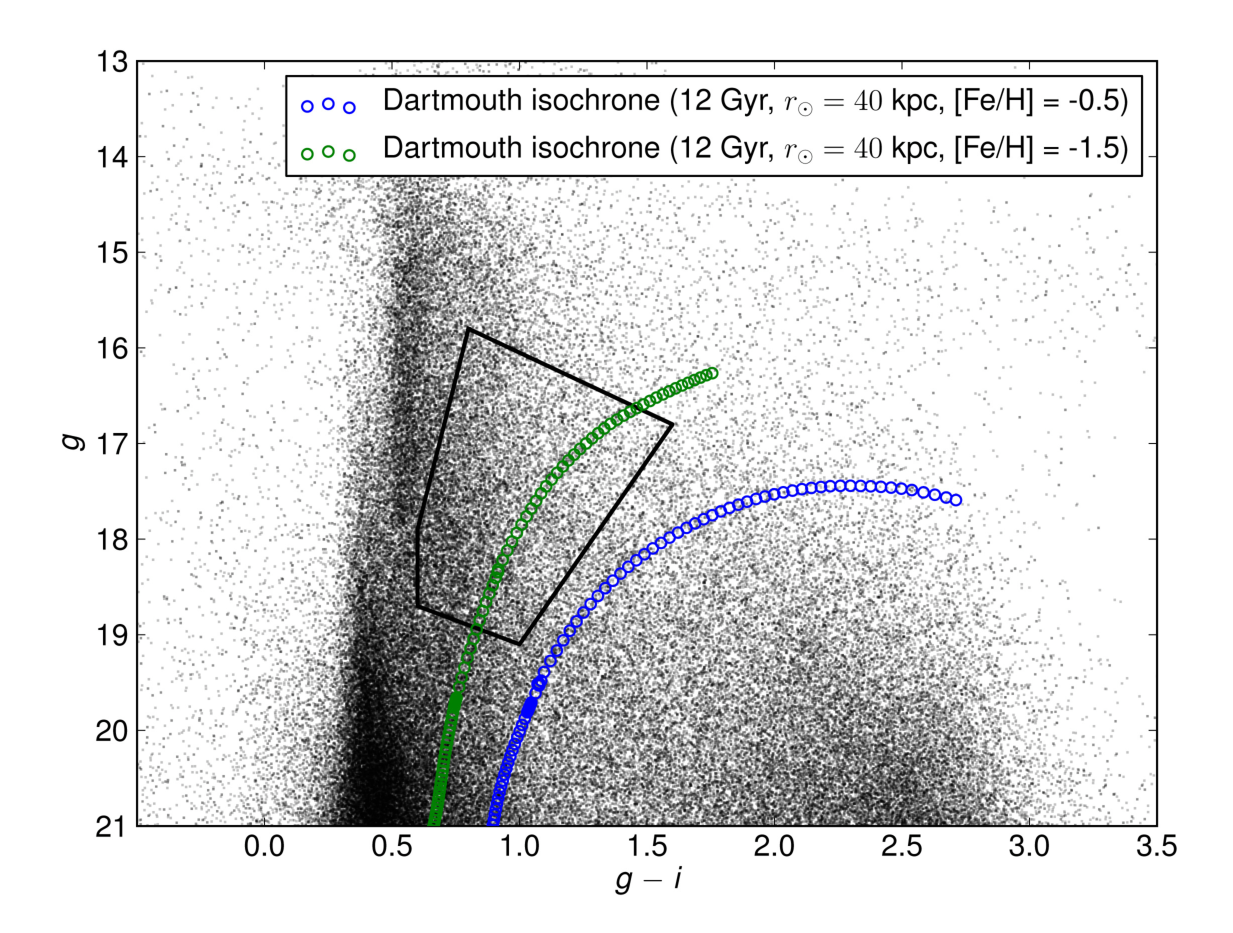
\includegraphics[width=9.2cm,height=6.8cm]{./figures/cmd.eps}
	\caption{Colour-magnitude diagram of the observed regions, illustrating the colour selection box.}
	\label{fig:cmd-target-selection}
\end{figure}

\noindent In order to specifically target K-giants, we have chosen candidates within the colour selection box
	
	\begin{eqnarray}
				0.6 <& (g-i)_o &< 1.7 \nonumber \\
				15 <& i_o &< 18 \\
		-15(g-i)_o + 27 <& g_o &< -3.75(g-i)_o \nonumber
	\end{eqnarray}
	
	
This selection region is illustrated in the colour magnitude diagram in Figure \ref{fig:cmd-target-selection}. Within this colour selection window, halo field dwarfs are expected to contaminate the sample due to their similarity in colours. Although K-dwarfs are difficult to distinguish photometrically, we can spectroscopically separate these through the absorption strength of the Mg 5180 \AA\, gravity-sensitive triplet (see \S\ref{sec:dwarf-giant-separation}).



	
	\section{Observations}
	\label{sec:observations}
	
	Our targets were observed in multiple runs using AAOmega on the 3.9-m Anglo-Australian Telescope (now the Australian Astronomical Telescope) at Siding Springs Observatory in New South Wales, Australia. AAOmega is a double-beam, multi-object fibre-fed spectrograph covering a two degree field of view. The targets were observed in normal visitor mode during two runs in April 2009. Throughout all observations, sufficient sky and guide fibres ($\sim 30$ and $7-8$ respectively) were allocated to ensure optimal sky subtraction and astrometry.
	
	The beam was split into the red and blue arms using the 5700 \AA\,dichroic. The 580V grating in the blue arm was used to provide giant/dwarf separation by measuring the absorption strength of the 5180 \AA\,Mg feature. The 580V grating yields spectra between 370-580 nm, with a resolution of $R = 1300 \AA$/px. In the red arm we used the slightly higher resolution (R$\sim$4400) 1000I grating which covers the spectral range between 800-950 nm. This coverage includes the Ca II infrared triplet, which is used for radial velocity measurements and metallicity estimations. To minimise scattered-light cross talk between fibres, the objects of each each configuration were limited to 1.5 magnitudes in range. Globular clusters NGC 5024, 5053 and 5904 were observed as radial velocity and metallicity standards, and no telluric standards were observed as telluric features do not affect the spectral features we are interested in.

	The data was reduced using the 2\textsc{DFDR} pipeline. After being flat-fielded the sky spectrum was subtracted using the median of the sky fibres and a carefully examined sky line list. The fibres were throughput calibrated, and wavelength calibration was achieved from arc lamp exposures between each set of science fields. Three thirty minute object exposures for each faint ($g > 16$) science field, and twenty-five minute exposures for bright ($g < 16$) field were taken to assist with cosmic ray removal.


	\section{Dwarf / Giant separation}
	\label{sec:dwarf-giant-separation}

	Photometric similarities in K-type giants and dwarfs will result in substantial contamination in our sample by dwarfs. In order to discriminate between these samples we have used the gravity-sensitive Mg feature at  5180 \AA. Our resolution is sufficient that this triplet is not blended and can be fitted with the sum of three Gaussian profiles. The Mg feature equivalent width is taken as the sum of the widths of each profile. One would expect a broader profile, in dwarf stars where the surface gravity is higher than that of giants. A blue spectra comparison between a giant and dwarf star is illustrated above in Figure \ref{fig:dwarf-giant-comparison}. The distinction in profile width is evident in Figure \ref{fig:dwarf-giant-separation}, which also demonstrates our separation line between giants and dwarfs. Contaminating dwarfs populate the dominant branch with a broader Mg profile, and K-giants populate the less-distinguishable lower branch. We identify 185 giants in this sample, and calculate the contamination of our input sample as 91\% dwarfs.
	
	\begin{figure*}[t!]
	\centering
	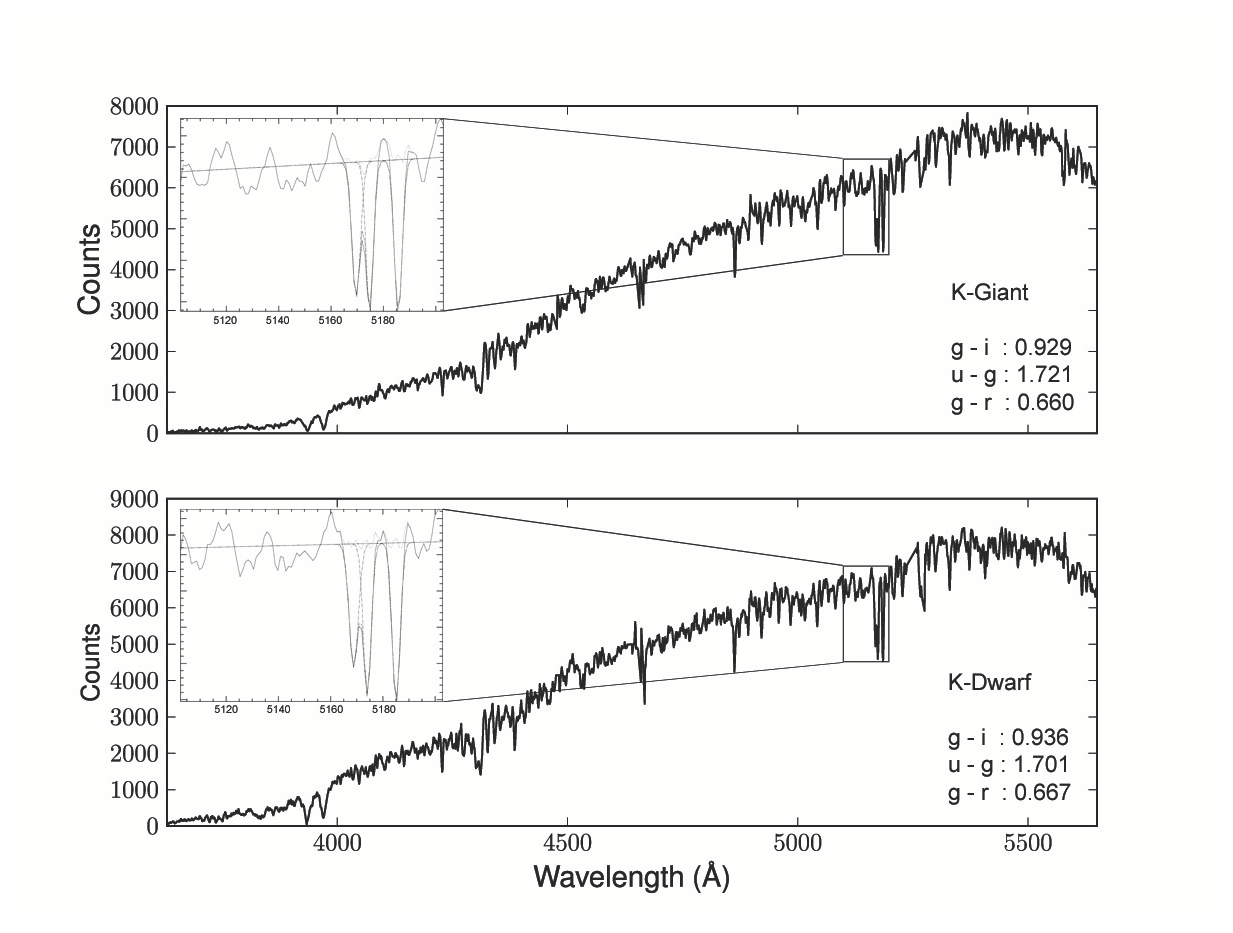
\includegraphics[width=18.4cm]{./figures/spectra.eps}
	\caption{Blue arm spectra for a K-type giant (top) and dwarf (bottom) star, highlighting the difference in the gravity-sensitive Mg 5180 \AA\, absorption profile.}
	\label{fig:dwarf-giant-comparison}
\end{figure*}
	
	%91 % is everything else. dwarfs is probably ~90% because some are identifiable carbon stars.
		
	\begin{figure}[h!]
		\centering
		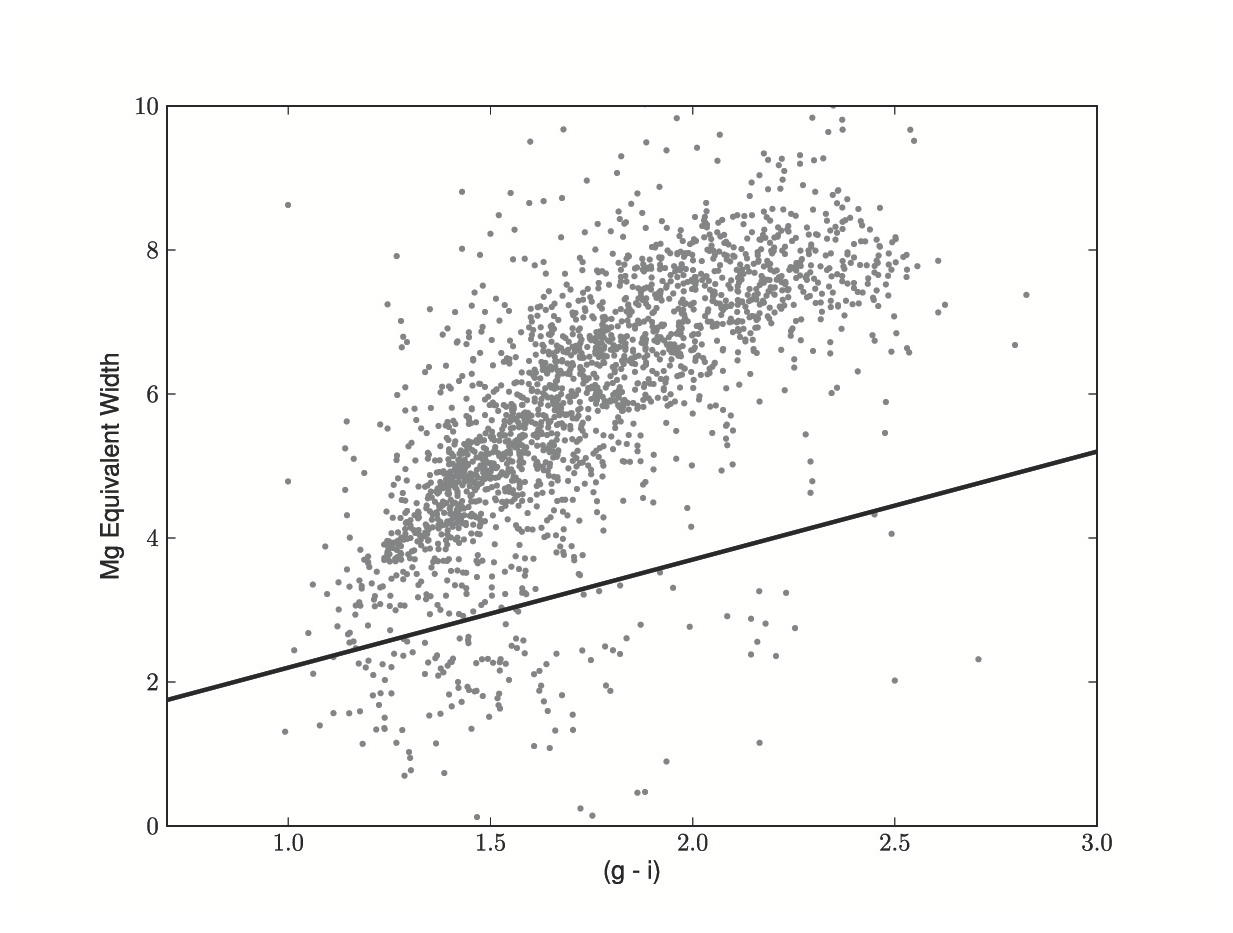
\includegraphics[width=9.2cm]{./figures/dwarfgiant_copy.eps}
		\caption{Equivalent width of the Mg 5180 \AA\ feature shown against the $g\,-\,i$ colour. The thick line is used to separate our dwarfs from giants. Field dwarf contaminants are largely illustrated in the dominant upper branch, and giant stars populate the lower horizontal branch.}
		\label{fig:dwarf-giant-separation}
	\end{figure}
	
	
	\section{Radial Velocities}
	\label{sec:kinematics}
	
	We have used the Ca triplet absorption lines at 8498, 8542 and 8662 \AA\, to measure radial velocities. These lines are strong, easily identifiable  (Figure \ref{fig:spectra}a) in RGB stars even at low resolution, and their prominence allows us to determine accurate radial velocities even with low signal-to-noise data. Our data has been cross-correlated with typical synthetic spectra of a K-giant ($T_{eff} = 4500$ K, $\log{g} = 0$, [Fe/H] $= -1.5$), and heliocentric corrections were made. Radial velocity measurements made on the standard stars in our globular clusters match up well (within 3 km s$^{-1}$) with the catalogue of \citet{Harris_1996} (2010 edition). Many of our targets were observed on multiple fields, which allows us to calculate the internal measurement error. The differences between multiple measurements of the same target were tabulated, and as expected form a half-normal distribution (Figure \ref{fig:multiple-kinematics}). The FWHM of this curve is +7.16 km s$^{-1}$. Kinematically 'cold' structures are typically identifiable if their peak signature has a FWHM of $< 8 $km s$^{-1}$, thus our intrinsic measurement error is small enough to identify cold substructures.
	
	\begin{figure*}[t!]
		\centering
		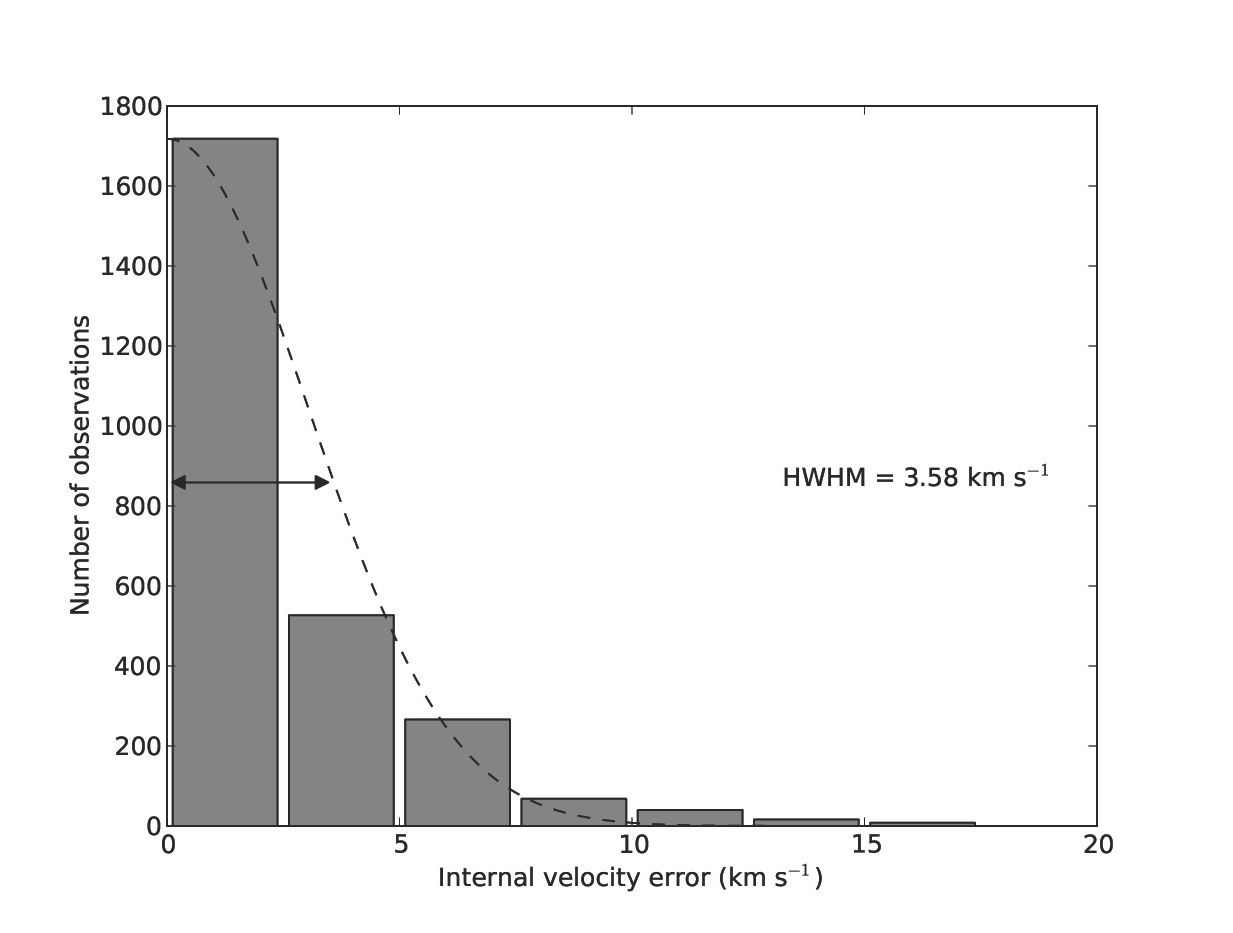
\includegraphics[width=18.4cm]{./figures/vel_error.eps}
		\caption{Internal radial velocity errors between multiple measurements of the same star. This sample includes all targets (dwarfs and giants) that were observed more than once.}
		\label{fig:multiple-kinematics}
	\end{figure*}
	
	In order to compare our kinematic results in a homogenous manner, we have translated our observed line of sight velocity to a galactocentric frame. We have adopted the circular velocity of the Local Standard of Rest (LSR) at the Sun as 220 km s$^{-1}$ \citep{Kerr;Lynden-Bell_1986} and accounted for the Sun's peculiar velocity to the LSR by using 16.5 km s$^{-1}$ towards $l = 53^{\circ}, b= 25^{\circ}$ \citep{Mihalas;Binney_1981}. The corrected line of sight velocity is then given by,
	\begin{align}
		V_{GSR} =  \,&\,V_{OBS} + 220\sin{l}\cos{b} + 16.5  \\
		 			&\,\, \times[\sin{b}\sin{25} + \cos{b}\cos{25}\cos{(l - 53)}] \nonumber
	\end{align}

\noindent where $V_{OBS}$ is the heliocentric corrected observed line of sight velocity.

	A caveat to this reference transformation is that previous authors in the literature have used slightly different formulae to transpose their kinematics to a galactocentric rest frame. This will result in a systematic shift in all corrected velocities between two authors using varied equations, and the level of the shift is purely dependent on the Galactic location of the observations taken. Impacts from this variation are discussed later in the text.

 
		
\section{Metallicities}
	\label{sec:metallicities}
	We have further used the Ca II triplet (CaT) lines to obtain approximate metallicity abundances  for our giant stars. Through measuring the profile width (W') of the CaT absorption lines, we can ascertain a metallicity determination using their magnitude above the horizontal branch as a calibrator. This technique was originally empirically described for individual stars \citep{Armandroff;Da-Costa_1991}, and has been extended to globular cluster members \citep{Rutledge;Hesser;Stetson_1997}, RGB stars and dSph members \citep{Battaglia;et-al_2008}. A spectroscopic analysis using VLT/FLAMES observations of RGB stars from composite populations led\citet{Battaglia;et-al_2008} to conclude, that a calibrated CaT-[Fe/H] relationship can be confidently used in composite stellar populations. However, a systematic trend is present where metallicity is overestimated by $\sim0.1$ dex at low metallicities ([Fe/H] < -2.2) and underestimated by $\sim0.1-0.2$ dex at higher metallicities ([Fe/H] > -1.2). \citet{Battaglia;et-al_2008} indicate higher Ca abundances may affect the CaT W' sufficiently to cause this trend, although [Fe/H] is the certain dominant factor contributing to the CaT W'. Nevertheless the CaT-[Fe/H] relationship is strong for RGB stars in composite populations (as observed here) above the horizontal branch within the range $-2.5 < $[Fe/H]$ < -0.5$.
	
The calcium-metallicity association is linear. The sum of equivalent widths of the CaT lines is scaled to form a 'reduced EW' (W'), which is calibrated by the stars magnitude above the horizontal branch ($V - V_{HB}$). This technique is only applicable for stars brighter than the horizontal branch ($V - V_{HB} > 0$). There is some discussion in which combination of the three CaT lines should be used. In this work we have taken the total equivalent width as the sum of the two stronger Ca lines ($\lambda_{8542}$, $\lambda_{8662}$). The weakest Ca line is usually the most unreliable when calculating equivalent width due to limited S/N and the possibility of residual sky-line contamination. Moreover, following a comparison of scaling relations between CaT and [Fe/H], \citet{Battaglia;et-al_2008} found using only the two strongest lines (as \citet{Tolstoy;et-al_2001} had done) was the most robust. As such, we have adopted the best-fitting relationship found by \citet{Battaglia;et-al_2008} for this work. The reduced EW is calculable by

\begin{eqnarray}
	\textstyle\sum{W}\, &=& EW_{8542} + EW_{8662} \\
	W' &=&\textstyle\sum{W} + 0.64\left(\pm 0.02\right)\left(V-V_{HB}\right)
\end{eqnarray}

\noindent and the metallicity linearly varies with the reduced EW such that,

\begin{equation}
	\text{[Fe/H]}_{\text{CaT}} = (-2.81 \pm 0.16) + (0.44 \pm 0.04) W'
	\label{eq:feh-cat}
\end{equation}


Using this calibration, our globular cluster standard stars have metallicities that match well with the \citet{Harris_1996} catalogue (2010 edition). When applying this technique to our K-giants, the difficulty is that the magnitude of the horizontal branch ($V_{HB}$) is not easily distinguished. $V_{HB}$ varies between stellar systems, and is dependent on the heliocentric distance and morphology of the stellar environment. This is a composite population; some stars are members of the Sgr stellar stream, others are members of the VOD/VSS, all superimposed upon field stars. Ideally we would want to uniquely identify each star to a stellar system and ascertain the horizontal branch magnitude. We can identify substructures kinematically, but we cannot differentiate halo stars. However, in our observed region there are known, dominant structures. The Sagittarius stream dominates our negative $V_{GSR}$ population, and our positive kinematic space is largely comprised of members from the VOD. As such we have kinematically separated our population at $V_{GSR} = 0$ into two samples to ascertain $V_{HB}$ for the two most dominant populations; Sgr and the VOD. Although this technique introduces a (known) systemic effect, it is the most useful way to accurately deduce the metallicity distribution. Statistically the most dominant [Fe/H] bin in each sample will be evident, and field halo stars or members from different substructures, will only add noise to the distribution.

\# rr lyrae table for 

The horizontal branch magnitude for the VSS has been ascertained from RR Lyrae observations by \citet{Prior;et-al_2009a}. Four of their RR Lyrae observations are proposed VSS members based on their galactocentric velocities, and the properties of these observations are listed in Table \ref{tab:prior-rrls}. The horizontal branch magnitude for all our K-giants with positive galactocentric velocities is taken as the median V-band magnitude of these four RR Lyraes, and calculated as $V_{HB} = 17.13$.

In order to determine the horizontal branch magnitude for the Sgr members a different technique has been used. The $V_{HB}$ of the dwarf progenitor is known, but it cannot be used for members along the stream, as the branch apparent magnitude is age- and distance-dependent. (\#citation needed) measured distances for 
	
%	Classical calibrations between CaT-[Fe/H] have used the magnitude above the horizontal branch as the dependent variable (cite me). The magnitude of the horizontal branch varies between stellar systems, and is dependent on heliocentric distance and the morphology of the system \citep{Harris_1996}. To reduce systematic errors between measurements, the same calibration ought to be used on all stars within our sample. However the stars examined here presumably originate from multiple, complex stellar environments and one cannot expect their horizontal branch morphologies to be the same. As our structures are identifiable through their kinematics, we could use known distances to many of these substructures in order to derive a $V_{HB}$ for each system. Although our substructures are recognisable, there is significant overlap between features which makes the kinematic selection windows of features ambiguous to chose at best. In contrast the absolute magnitudes $M_I$ and $M_V$ introduce a much smaller systematic effect. Although \citet{Cole;et-al_2004} showed the effect of different ages of RGB stars is a negligible source of error for metallicities derived from the CaT calibration, \citet{Carrera;et-al_2007} shows it is advantageous to use $M_I$ (instead of $M_V$) for the calibration because it is much less sensitive to age effects. With these caveats in mind, we have decided to use the $M_I$-[Fe/H] calibration. As such, Equation \ref{eq:starkenburg-metallicity} becomes
		
% A caveat to the Ca II line strength-[Fe/H] relationship is that it is empirically defined and not entirely well understood.

% Globular cluster stars used for the calibration are typically drawn from a single population, however the stars examined here are drawn from multiple, sometimes unknown, origins. Moreover, differing [Ca/Fe] ratios between multiple globular clusters is expected to affect the strength of the Ca lines. 
		
	%A comparison between multiple calibrations between groups yields close correlations between the techniques \citep{Battaglia;et-al_2008}.
%	Although the origins of the VOD and many of the nearby spatial substructures is unknown, many of the targets examined may have origins in the Sagittarius dSph galaxy. It is appropriate to use calibrations made on RGB stars, and as such the technique described within \citet{Starkenburg;et-al_2010} is implemented here. Using their relationship, the equivalent width sum  to determine an abundance for either [Fe/H] or [Ca/H]. Calibrations have been provided between three different absolute magnitudes; $\left(V-V_{HB}\right)$, $M_V$ or $M_{I}$ (Johnson-Cousins). Coefficients for the functional form of the equation (Eq. \ref{eq:starkenburg-metallicity}) depend on the absolute magnitude-abundance calibration used. The term $V_{HB}$ specifies the $V$ magnitude of the horizontal branch, and as these calibrations are only valid for RGB stars, \citet{Starkenburg;et-al_2010} stresses they should not be applied to stars outside $-3 < \left(V-V_{HB}\right) < 0$, $-3 < M_V < 0.8$, or $-4 < M_I < 0$.
		
%	\begin{eqnarray}
%		\label{eq:starkenburg-metallicity}
%		\text{[Fe/H]} &=& a + b \times M_X + c \times EW_{(2+3)} \\
%				      &\,   &\,\,\,\,\,     + d \times EW_{(2+3)}^{-1.5} + e \times EW_{(2+3)} \times M_X \nonumber
%	\end{eqnarray}



	\section{Discussion}
	\label{sec:discussion}

	Along our line of sight, the spatial region examined in this paper incorporates the superposition of multiple substructures, some which may be inter-related. To facilitate a logical flow of discussion, these substructures ought to be separated and identified first. 	
		
		\subsection{Substructure Identification}
		\label{sec:substructure-identification}
		
		When discussing our data with respect to stellar streams and substructures within the halo from here, we are referring only to K-type giants.  Dwarfs are too faint to be found at a sufficiently large distance where we are exploring substructures. Given a randomly selected distribution of stars, we ought to expect their galactocentric velocities to be representative of the halo if the sample is sufficiently large. A significant kinematic deviation from a canonical halo population is the classic signature of a co-moving group. In order to quantitatively compare the kinematics of stars in our sample to a halo distribution, we have represented our galactocentric velocities with a generalised histogram (Figure \ref{fig:velocity-histogram}). The generalised histogram represents each data point with a Gaussian kernel of an equal bandwidth (deviation). The selection of bandwidth is important and can over- or under-smooth data and misrepresent results if chosen incorrectly.
		
		In order to gain an approximation for the bandwidth selection we have looked at stars in our dataset with repeated observations. Since we are investigating the systematic accuracy of our velocity measurements, and not focussed on substructure identification, we can include K-type dwarfs in our multiple measurement sample in order to gain a more accurate representation of the systemic measurement error. A histogram showing the number of repeated observations, as well as the errors in repeat velocity measurements between stars is shown in Figure \ref{fig:multiple-kinematics}. The kinematic errors between multiple measurements summate to a half-normal distribution with a FWHM of 7.16 km s$^{-1}$. This represents the minimum bandwidth we can feasibly use to represent our data. We have opted for a bandwidth value of 10 km s$^{-1}$ for the generalised histogram in Figure \ref{fig:velocity-histogram}.
	
		
\begin{figure}[h]
	\centering
	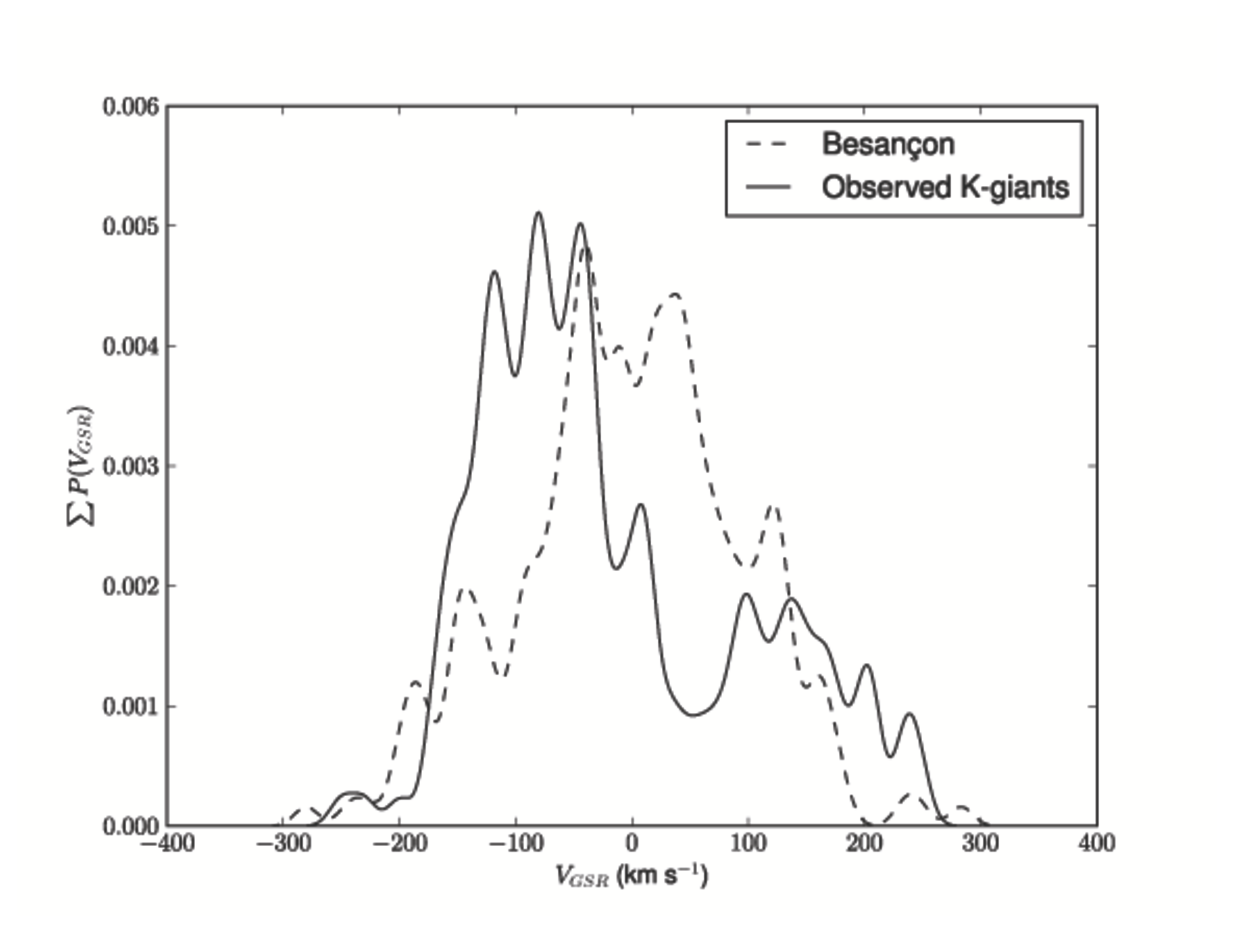
\includegraphics[width=9.2cm]{./figures/besancon_copy.eps}
	\caption{Generalised histogram of $V_{GSR}$ for the sample K-type giants, highlighting their significance against the predicted observations by the  Besan\c{c}on model for this spatial region.}
	\label{fig:velocity-histogram}
\end{figure}

				




	As evident in Figure \ref{fig:velocity-histogram}, there are significant ($> 3\sigma$) tight kinematic signature peaks. As previously noted, the fields observed here have numerous identified overlapping substructures, and potentially many more which have not been disentangled. The most dominant of these features (Feature A) is that within the bin of $-200 < V_{GSR} < -10$, where we would expect some halo contaminants, especially at the more positive velocity end of the bin. This wide spread in kinematics has a bulk overall dominant signature well in excess of the halo. We attribute this wide, yet significant kinematic peak to a single membership; the leading arm of the Sagittarius tidal tail. 	
		

	One could argue that the generalised histogram presented in Figure \ref{fig:velocity-histogram} is over-smoothed, and perhaps three independent kinematic signatures are present within this bin. This is indeed possible, however using the minimum bandwidth possible (6.76 km s$^{-1}$) without over-interpreting the data, the shape of the peaks remains consistently narrow, although no firm conclusions can be drawn about possible sub-populations. It is also possible that these peaks are artefacts of the sampled population, and would not appear in the same positions given a different (or larger) sample size. Representing the data as a generalised histogram with an appropriate bandwidth is a methodical way to eliminate such projected artefacts, and they ought not to be statistically significant in Figure \ref{fig:velocity-histogram}. Alternatively we present evidence (see \S\ref{sec:sgr-peak-analysis}) suggesting these features are indeed real, and not consequences of the sampled distribution. Albeit they have a wide kinematic distribution, may still be members of a single population.
		
	Feature B is our next most evident substructure at $V_{GSR} = +130$ km s$^{-1}$, which we attribute to the Virgo Stellar Stream, as other authors have \citep{Newberg;et-al_2007, Prior;et-al_2009a}. These members in our 130 km s$^{-1}$ bin ($120 < V_{GSR} < 140$ km s$^{-1}$) are coincident in spatial position, velocity, and metallicity (see \S\ref{sec:the-vss}) with previously reported values of the VSS obtained by F turnoff and BHB stars \citep{Newberg;et-al_2007} and RR Lyrae stars \citep{Prior;et-al_2009a}.
		
		
	\subsection{Feature A \--- Sagittarius Debris}
	
	The tidal debris of Sagittarius wraps around the entire Galaxy, and these tails have been extensively traced \citep{Belokurov;et-al_2006,Newberg;et-al_2007,Yanny;et-al_2009}. It is useful to see how the bounds of our observed fields spatially overlap with the Sagittarius stream (and other substructures), so we can provide a useful analysis. Figure \ref{fig:sgr-field-of-streams} shows the bounds of our observed region overlayed upon a panoramic projection of the Sagittarius stream and the 'Field of Streams' from \citet{Belokurov;et-al_2006}. This is a crowded region of globular clusters, substructures and overlapping stellar streams, primarily populated by the Sagittarius Northern arm. The bifurcation in Sagittarius \citep{Belokurov;et-al_2006} is evident here, and our observed fields overlap with the the more southern Branch A.
			

	\begin{figure*}[t]
		\centering
		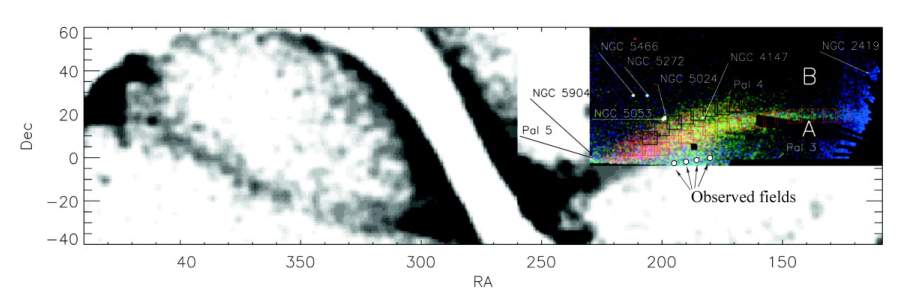
\includegraphics[width=18.4cm]{./figures/belokurov2006.eps}
		\caption{Spatial bounds of our observed fields outlined upon a panoramic view of the Sgr stream, using the 2MASS M giants of \citet{Majewski;et-al_2003} with SDSS stars. This plot is an adaptation of Figure 2 in \citet{Belokurov;et-al_2006}.}
		\label{fig:sgr-field-of-streams}
	\end{figure*}
	
		
	Simply from a spatial perspective, we expect Sagittarius debris to dominate our data. \textit{N}-body models of the Sagittarius stream suggest highly negative velocities in this region \citep{Law;et-al_2005,Law;Majewski_2010}, which has led several authors \citep{Yanny;et-al_2009, Prior;et-al_2009b}, who have observed co-moving groups with highly negative kinematic signatures in nearby fields, to attribute these as members of Sagittarius.  Our generalised histogram in Figure \ref{fig:velocity-histogram} demonstrates a bulk kinematic signature, well in excess of the halo. Smaller kinematic signatures are difficult to distinguish, and determining their membership can be arduous. The extent of the kinematic signature here can only result from a dominant population, such as Sagittarius. 
		
		
	\subsection{Sagittarius Debris: Comparison to Models}
		
	The consequential tidal tails from the Sgr-Milky Way interaction has been modelled by many groups \citep[e.g. ][]{Helmi_2004, Law;et-al_2005, Law;Majewski_2010}. In order to further investigate the spatial coverage and kinematics from our sample of stars attributed to Sagittarius, we have compared our sample of K-giants with the constant flattening spheroidal models of LJM05 and the more recent tri-axial model of LM10. The simulated data output from these is readily available online\footnote{http://www.astro.virginia.edu/$\sim$srm4n/Sgr/}, and their released models have the best-fitting parameters for each model classification (prolate, spherical, oblate and tri-axial). Simulations are matched to the 2MASS M-giant sample, which provides an all-sky view of the Sgr stream. These are the only simulations available which make use of an all-sky data set, and comparisons between each model will be more consistent than comparing models between different authors.
		
		\citet{Law;et-al_2005} describe the Milky Way as a smooth, rigid potential and represent Sgr with $10^5$ self-gravitating particles. The Galactic potential is represented with three primary components; a \citet{Miyamoto;Nagai_1975} disk, a Hernquist spheroid and a logarithmic halo. The models of LJM05 have a constant degree of flattening, $q$, whereas the more recent LM10 tri-axial model has a minor/major axis ratio $(c/a)_\Phi = 0.72$ and an intermediate axis ratio $(b/a)_\Phi = 0.99$ at radii $20 < r < 60 $kpc. In models with constant flattening, three classification types were considered and the value $q$ was chosen from the best-fitting simulation type; prolate (constrained $q > 1; q = 1.25$ set), spherical ($q = 1.0$ set), and oblate (constrained $q < 1; q = 0.80$ set). Their models integrate over 3 Gyrs (around four orbits) and predict heliocentric distances and galactocentric velocities, and adopt a heliocentric Sgr coordinate system with longitude $\Lambda_\odot$ and latitude $B_\odot$, as defined by \citet{Majewski;et-al_2003}. The Sgr core is centered at $\Lambda_\odot = 0^\circ$, and latitude plane is defined by the best-fitting great circle of the Sgr debris. For comprehensive details of the simulations the reader is referred to the papers of \citet{Law;et-al_2005, Law;Majewski_2010}. To illustrate the spatial distribution simulated by the Sgr tidal tails, Figure \ref{fig:law-spatial} shows the simulated particles from the LJM05 and LM10 models, and our observed fields are outlined in black. 
		
		\begin{figure}[h]
			\centering
			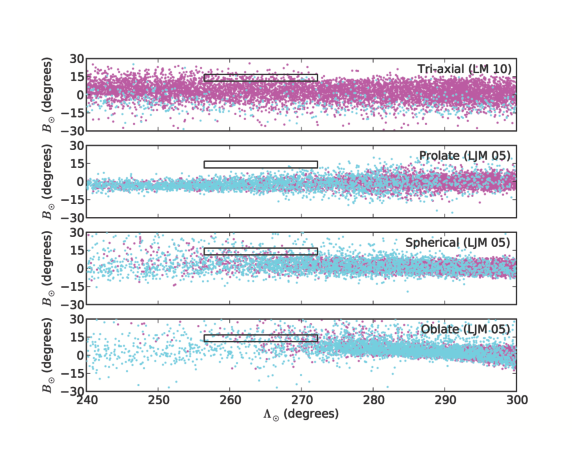
\includegraphics[width=9.2cm]{./figures/law_spatial_copy.eps} 
			\caption{The bounds of our observed area is outlined in black against the simulated particles from multiple \textit{N}-body simulations by LJM05, LM10. The particles are colour-coded by their peri-centric passage following the same convention by \citet{Law;Majewski_2010} (magenta; previous passage, cyan; oldest observable passage). \\ A colour version of this plot available in the online journal.}
			\label{fig:law-spatial}
		\end{figure}
	
	The Northern leading arm of Sgr is particularly sensitive to both kinematic and spatial changes in the shape of the Milky Way dark halo. To evaluate how well models predict the position and kinematics of the Sgr debris, we require either a large set of accurate stellar kinematics and distances, or targeted regions of the stream where a change in the shape of the dark halo results in significantly different simulated positions and kinematics. The latter is particularly the case for our fields when compared to the spatial positions predicted by the prolate model (Figure \ref{fig:law-spatial}).  All other models predict the Sgr stream to pass directly through our fields, however the prolate model predicts no particles directly in our fields, and when we extend a rectangle bounded by the edges of our fields only two particles are found. Spatially the prolate model predicts the Sgr stream to pass more southward (in $B_\odot$) than our observed fields. If this prolate halo model is a true representation of the Sgr debris, this does not exclude the potential of finding some Sgr debris in our fields. However it strongly suggests that if the dark halo is indeed prolate, and the LJM05 prolate model is a good representation of the halo, Sgr would not be the dominant observed population as we see in our fields.
	
	In comparison, the tri-axial, spherical and oblate models predict varying amounts of particles from previous peri-centric passages to pass through our observable region. To adequately evaluate the model predictions of Sgr debris, a kinematic comparison between the predicted and observed values is necessary. As the prolate model has only two simulated particles within our observable bounds there is no qualitative kinematic comparison to be made for this model.
	
	The number of predicted particles in our observed region is different for each model, and as the amount will not necessarily reflect the size of our observed sample. Consequently the kinematics for each model have been represented as a generalised histogram (Figure \ref{fig:law-vel-compare}). For consistency all simulation output and observed data has been convolved with a Gaussian kernel of 10 km s$^{-1}$; the bandwidth used for the generalised histograms with observed data. A generalised histogram is an effective method to evaluate the model predictions, because the size the overall distribution is scaled such that the integral of each distribution is unity. Therefore populations of different sizes (i.e. our observed sample and the varying size of each simulation output) are scaled appropriately so we can evaluate the kinematic signatures. One caveat of this technique is that the relative size of each sample must be acknowledged when evaluating the predictions made by a model. A narrow distribution \--- which may perfectly match the observed data \--- may simply be a consequence of an extremely small sample size, yielding an ineffective comparison. Indeed if we included a comparison with the prolate model the entire distribution may appear to represent the observed data closely in a qualitative sense, however that distribution would be composed from a mere two simulated particles.
	

\begin{figure*}[t!]
	\centering
	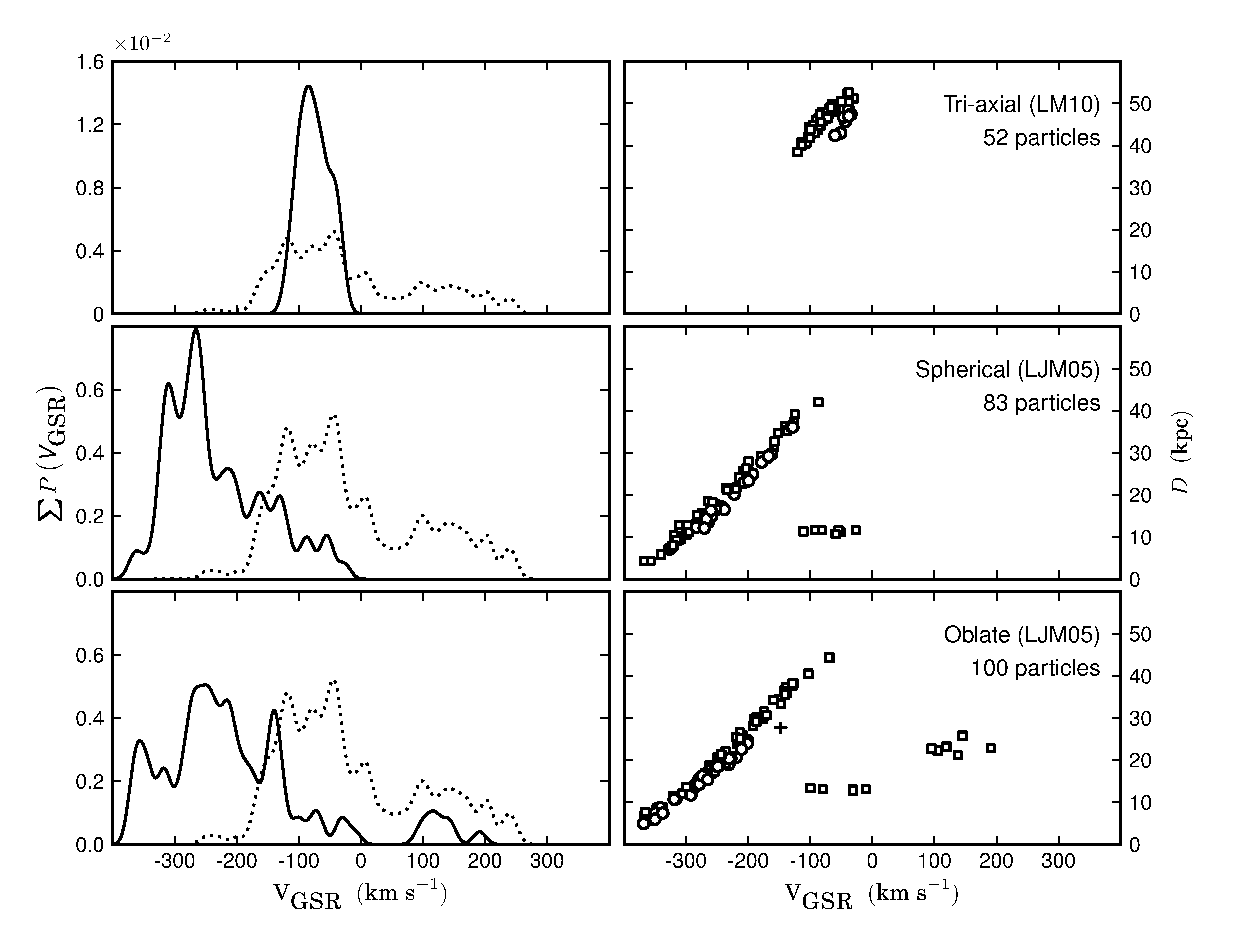
\includegraphics[width=18.4cm]{./figures/lawvelcompare-bw.eps}
	\caption{A generalised histogram (left) of the galactocentric rest frame velocities in our sample (dotted line) compared to the velocities from the \textit{N}-body models of LJM 05, LM 10 of particles within the same spatial coverage and age of our observed sample (solid lines). The model particles used to generate each velocity histogram are shown on the right in velocity-heliocentric distance space, and they are labelled by their recency of passage. A plus ($+$) denotes debris from the current peri-centric passage by Sgr, circles ($\circ$) mark the previous passage, and squares ($\square$) represent debris from two previous passages.}
	\label{fig:law-vel-compare}
\end{figure*}


	With this caveat in mind we have also shown the simulated particles predicted within our observable bounds on a kinematic-distance scale in Figure \ref{fig:law-vel-compare}. Clearly, in this small region there is debris from multiple passages predicted along the line of sight, and as such particles have been marked by their recency of peri-centric passage. Distinguishing particles by their peri-centric age allows us to qualitatively differentiate relative kinematic contributions of the stream by their recency of passage.  In all three models, the Northern arm is clearly distinguishable, albeit the tri-axial model has a much tighter sequence in velocities. This is attributed to the position of the predicted pericenter. The tri-axial model predicts a pericenter almost precisely where our fields were observed, whereas the spherical and oblate model predict a large wrap of the stream along the line of sight, resulting in a large spread in kinematics and heliocentric distances.


		





	In our observed fields, the spherical and oblate models predict close-by debris with extremely highly negative galactocentric velocities. This signature is not representated in our data. The lowest observed velocity is $\sim -250$ km s$^{-1}$ and we have only two observations less than $V_{GSR} < -200$ km s$^{-1}$. In contrast, in these two simulations the bulk predicted kinematic signature extends well below $V_{GSR} < -300$ km s$^{-1}$. If the dark matter potential is well-represented by either of these LJM05 simulations then this discrepancy must be reconciled. 
	
	K-giants have a large range in absolute magnitudes, nevertheless nearby stars will appear brighter and may be brighter than the magnitude range of our observed targets. A colour-magnitude diagram for the Besan\c{c}on model data in this area is shown in Figure \ref{fig:besancon-cmd}a, which highlights the giant branch and includes an outline of our target selection criteria. The predicted distances to each of these stars along the giant branch is represented in Figure \ref{fig:besancon-cmd}b, which shows a predicted observable distance range for K-giants between X to Y kpc - as we would expect. Using this distance cut to exclude unobservable stars, we would lose some of our simulated particles in the most negative velocity region for each model in Figure \ref{fig:law-vel-compare}. However this constraint is insufficient to adequately explain the substantial velocity discrepancy between our observed data, and the LJM05 spherical/oblate models.
	
		
\begin{figure}[h!]
	\centering
	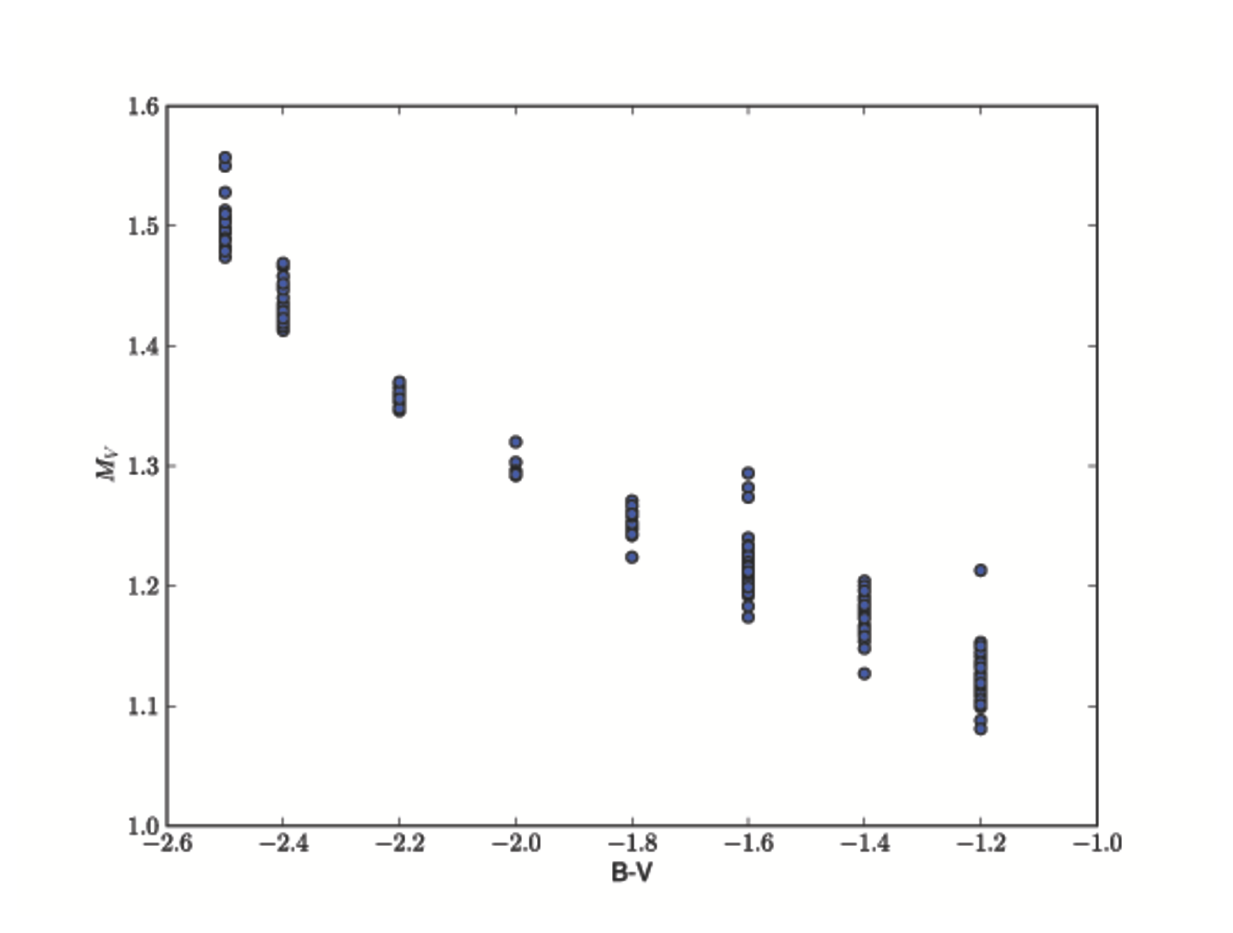
\includegraphics[width=9.2cm,height=7cm]{./figures/besancon-cmd_copy.eps}
	\caption{Colour-magnitude diagram using $M_V$ against $B-V$ from the Besan\c{c}on model in this area (left), illustrating the giant branch. The distances to those giant-branch stars are shown in the histogram on the right, representing the range of potential K-giant observable distances. }
	\label{fig:besancon-cmd}
\end{figure}

	These two models also illustrate a similarity signature at $\sim$12 kpc, with simulated particle velocities ranging between $-100 < V_{GSR} < 0$ km s$^{-1}$. This is the edge of a simulated crossing-point between different wraps of the stream, which occurs at $\sim12$ kpc and yields a wide range of kinematics focussed at a common distance. These particles (and the positive kinematic signature around $\sim$20 kpc in the oblate model), are relatively minor signatures when compared to the overall bulk signature of the Northern arm. If these signatures are present in our observed fields, their banality would prevent them from appearing as significant relative to either a normal halo population, or a halo population in addition to expected substructure material (e.g. the VSS, 12\fh4 clump, S297+63-20.5). As such we cannot use the edge particles of these nearby simulated wraps to discern substantial information regarding the dark halo of the Milky Way.

	In this region, the kinematic predictions of the tri-axial dark halo model best fit our observed data. However, the tri-axial model kinematics favour our data set, the predicted kinematic distribution from a tri-axial halo is much narrower than our observed sample. Our broad observed sample is unlikely to be a consequence from considerable halo members. The profile broadening in our sample extends most prominently at highly negative galactocentric velocities ($\sim -200$ km s$^{-1}$). Given any Gaussian-like population with a mean near zero, we would expect less halo members at high galactocentric velocities \--- positive or negative. One reconciliation for this profile discrepency may lie in the workings of the tri-axial model itself. Unlike the other models compared here from LJM 05, the tri-axial model does not reproduce the bifurcation observed in the Sgr stream \citep{Belokurov;et-al_2006} as recent studies prior to the model development suggested this may be an outcome from the internal dynamics within the progenitor, and not primarily resultant from the shape of the Milky Way dark halo\citep{Fellhauer;et-al_2006}. However, \citet{Penarrubia;et-al_2010} recently found no evidence for internal rotation in the remnant core of the Sgr dwarf sufficient enough to produce a bifurcation.


	The lack of bifurcation treatment in this model may explain the particularly narrow distribution predicted in this region. Other groups have observed the spatial disruption caused by the bifurcation, however whether a kinematic variation exists between branches is unclear. Given the kinematic interactions within the progenitor, and the gravitational influence of the halo, it is reasonable to suggest a kinematic disruption may consequent from the bifurcation. A comparative targeted study along each branch would be necessary to discern a kinematic disruption. The region observed here is on the southern edge of Branch A. Despite that, some overlap between the two branches is plausible, and we postulate that such a kinematic variation may explain the discrepancy between the predicted narrow distribution which peaks in concert with our data, and the broader observed profile. 
	
	


%The astute reader will notice in Figure \ref{fig:law-vel-compare} that the tri-axial model also predicts two wraps from different peri-centric passages in this region. The two are predicted to be close in distance, and if present they would be spatially indistinguishable in our fields. However there is a known metallicity gradient along the Sgr field \citep{cite-me}, and multiple metallicity sub-populations which vary in density along the wraps. One might expect then that if the tri-axial model by LM 10 is a good representation of the Sgr streams in this region, that we might see a bi-modal metallicity distribution in the Sgr-attributed members. Exploring this idea, Figure \ref{fig:sgr-metallicity-hist} demonstrates the metallicity distribution for all K-giant members with negative galactocentric velocities. Although this sample will contain halo members and contaminants, the dominant population is Sagittarius. No bi-modal distribution is observed, however this does not exclude the possibility; our metallicity accuracy ($\pm 0.3$ dex) would not be sufficient to discern stars from an immediately previous wrap ($\pm $N dex; cite-me). Moreover, members of the previous wrap would be sparsely populated in comparison to its younger counterpart.

\subsection{Sagittarius Debris: A Metal-Poor Population Uncovered?}
\label{sec:sgr-metal-poor}

\# To do.	
	\begin{figure}[h!]
		\centering
		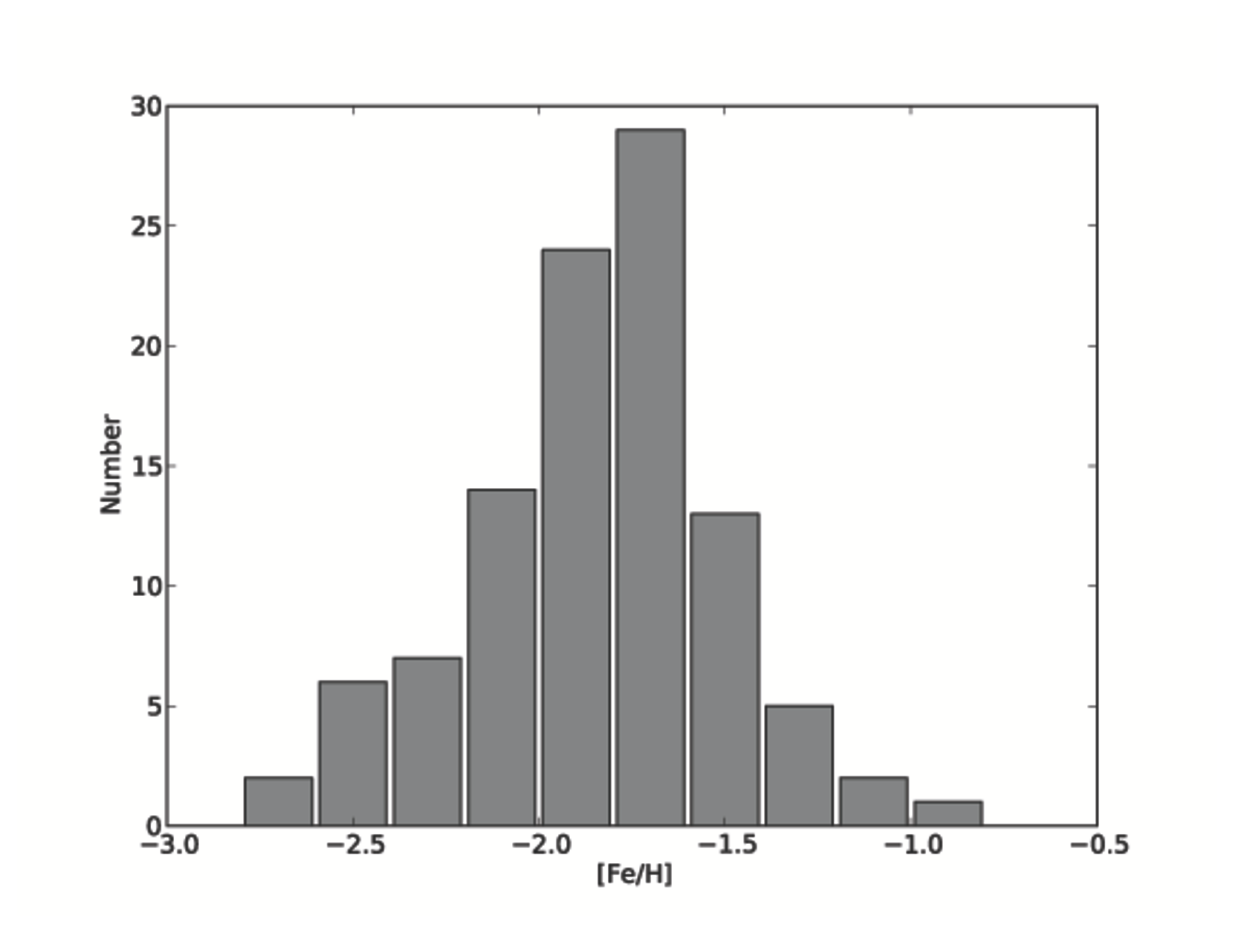
\includegraphics[width=9.2cm]{./figures/fehhist_copy.eps}
		\caption{Metallicity determinations for K-giants with negative galactocentric velocities; which are largely attributed to the Sagittarius Northern arm.}
		\label{fig:sgr-metallicity-hist}
	\end{figure}
	
	
\subsection{Sagittarius debris: Are the features at $-49$ and $-76$ km s$^{-1}$ related?}
\label{sec:sgr-peak-analysis}
			
	Our most dominant kinematic groups peaks at $V_{GSR} = - 49$ and $-76$ km s$^{-1}$. Intuitively one may wonder whether these two objects are observations of unique structures or a systemic artefact of a single structure. \citet{Vivas;et-al_2008} noted that the most populated group in their sample of BHB and RR Lyrae stars occurred within the bounds $-80 < V_{GSR} < -10$ km s$^{-1}$, and had a mean velocity of $V_{GSR} = -49$ km s$^{-1}$ with a standard deviation of 22 km s$^{-1}$. This sample comprised of nine RR Lyrae stars and five BHB stars. Metallicity measurements of the variables within the group yielded a mean metallicity of $\langle$[Fe/H]$\rangle$ = -1.72 dex with a standard deviation of 0.28 dex. In this region of high negative velocity\citet{Vivas;et-al_2008} expect relatively high contamination from unrelated halo stars and suggest this may skew their kinematics. However they state this does not account for the diffuse metallicity distribution. The spread is likely representative of the true population, and not caused by the contamination of non-members into an otherwise narrow distribution. 
	
\# As a comparison, our K-giants in the same galactocentric velocity range demonstrate a metallicity of X and a standard deviation of Y dex. \\
\# Is ours higher or lower? \\
\# Is there some selection metallicity effect when comparing K-giant derived metallicities to RR Lyraes? \\
\# ie would you expect RR Lyraes to be more metal poor because they are an older generation, etc \\
			
			
	The peak velocity signature at $V_{GSR} = -76$ km s$^{-1}$ has also been noted by others. \citet{Duffau;et-al_2006} observed BHB stars in this region and illustrated a slight peak in the bin $-80 \lesssim V_{GSR} \lesssim -50$ km s$^{-1}$. \citet{Newberg;et-al_2007} found a significant peak in the velocities of F-type stars at $-76$ km s$^{-1}$, which \citet{Vivas;et-al_2008} notes may be members of the $-49$ km s$^{-1}$ structure, given the errors. The RR Lyraes in the \citet{Vivas;et-al_2008} sample at $V_{GSR} = -49$ km s$^{-1}$ have a distance of $7.5 < D < 9.5$ kpc and using a conservatively faint absolute magnitude $M_g = +4.2$ for the \citet{Newberg;et-al_2007} sample, \citet{Vivas;et-al_2008} estimate the distance to the F-type stars would be around $11 \lesssim D \lesssim 14$ kpc. If these two features are related then their distance and kinematic discrepancies must be reconciled, and their spatial coverage is worthy of interrogation.

	\begin{figure}[h!]
		\centering
		\includegraphics[width=9.2cm,height=7cm]{./figures/blank.eps}
		\caption{The sky coverage examined in this data set which contains K-giants within our velocity bin ranges $-59 < V_{GSR} < -39 $km s$^{-1}$ (green squares) and $-86 < V_{GSR} < -66 $km s$^{-1}$ (blue circles), and the spatial coverage examined by other authors \citep{Duffau;et-al_2006, Newberg;et-al_2007} who separately noted the same peaks; illustrating the spatial overlap.}
		\label{fig:newberg-duffau-vivas-spatial}
	\end{figure}
			
		
	\citet{Newberg;et-al_2007} notes that their $-76$ km s$^{-1}$ feature is more pronounced in the fainter $(l, b) = (300^\circ, 55^\circ)$ field, although upon recognising the feature they note it is also seen in their more northerly plate at $(288^\circ, 62^\circ)$. The more spatially prominent region covered by \citet{Newberg;et-al_2007} was not observed by \citet{Vivas;et-al_2008}, so the spatial overlap between these authors could not be fully investigated. The spatial region covered by \citet{Duffau;et-al_2006} (which included the $-49$ and $-76$ km s$^{-1}$ features) ranged from (R.A., Dec.) $\approx$ (175 to 200$^\circ$, -2 to 0$^\circ$), which overlaps with this work and the fields by \citet{Newberg;et-al_2007} (Figure \ref{fig:newberg-duffau-vivas-spatial}). Our $-76$ km s$^{-1}$ group is most spatially concentrated within (R.A., Dec.) = (189 to 195$^\circ$, $-3.5$ to $-1.5^\circ$), which overlaps with the region where \citet{Duffau;et-al_2006} observed a similar peak and extremely close to the centroid where \citet{Newberg;et-al_2007} found their $-76$ km s$^{-1}$ peak of F-type stars.
			

		Although we uncover more stars from the $-49$ km s$^{-1}$ peak in this spatial region we also expect a higher contamination of halo stars in this sample. With that caveat in mind we can see the sample extending towards (R.A., Dec.) = ($180^\circ$, $0.5^\circ$), although there are only N stars here. Similarly we might expect that perhaps one of in the $-76$ km s$^{-1}$ group that are separated from the clump is a contaminant, or that the group is simply not as diffuse as the $-49$ km s$^{-1}$. A larger sample is favourable as it is problematic to distinguish or otherwise assign common membership to these moving groups based on their spatial coverage. However due to repeated measurements by multiple authors and given their kinematic dispersions, X km s$^{-1}$ for the $-49$ km s$^{-1}$ group and Y km s$^{-1}$ for the $-76$ km s$^{-1}$ group, this suggests these may be separate kinematic structures superimposed on one another. Further investigation in this region to explore this idea would be interesting.
			
			

	\subsection{Feature B \--- The Virgo Stellar Stream}
	\label{sec:the-vss}
	
	As previously mentioned, our observable region falls within the 'Field of Streams' where multiple stellar substructures and co-moving groups have been noted by several groups. The largest, most diffuse structure in this region is the VOD, stretching up to $\sim$1000 deg$^2$ across the sky \citep{Juric;et-al_2008}. One such smaller substructure which was distinguished from the general over-density of the VOD is the Virgo Stellar Stream \citep{Duffau;et-al_2006}. Several RR Lyrae stars were noted by \citet{Prior;et-al_2009a} with a common velocity of $V_{GSR} = 130$ km s$^{-1}$. This kinematic signature has been repeatedly observed in this region by other groups \citep{Newberg;et-al_2007, Prior;et-al_2009a}, and \citet{Prior;et-al_2009a} used measurements of RR Lyrae stars with the same kinematic signature to obtain a metallicity of [Fe/H] = -1.95 for the VSS. 
	
	% Discuss the VGSR = 100 discrepancy? %
	
	We cannot unequivocally state whether members of the VSS are present in our K-giant sample \textit{only} from looking at kinematic signatures alone. In Figure \ref{fig:velocity-histogram} there is a slight peak at $V_{GSR} = +130$ km s$^{-1}$, however this peak is not statistically significant. It is impossible to discern which, if any, members within the bin $120 < V_{GSR} < 140$ km s$^{-1}$ are potential VSS candidates. Kinematics of members in the bin are perfectly representative of randomly selected stars within the halo. The discrimination between halo and potential VSS candidates becomes more discernible when we explore metallicity measurements. Figure \ref{fig:velocity-metallicity} shows the velocities and metallicities for all of our K-giant candidates. % Discuss the sharp jump at VGSR = 0 and what implications that has. %
	
	\begin{figure}
		\centering
		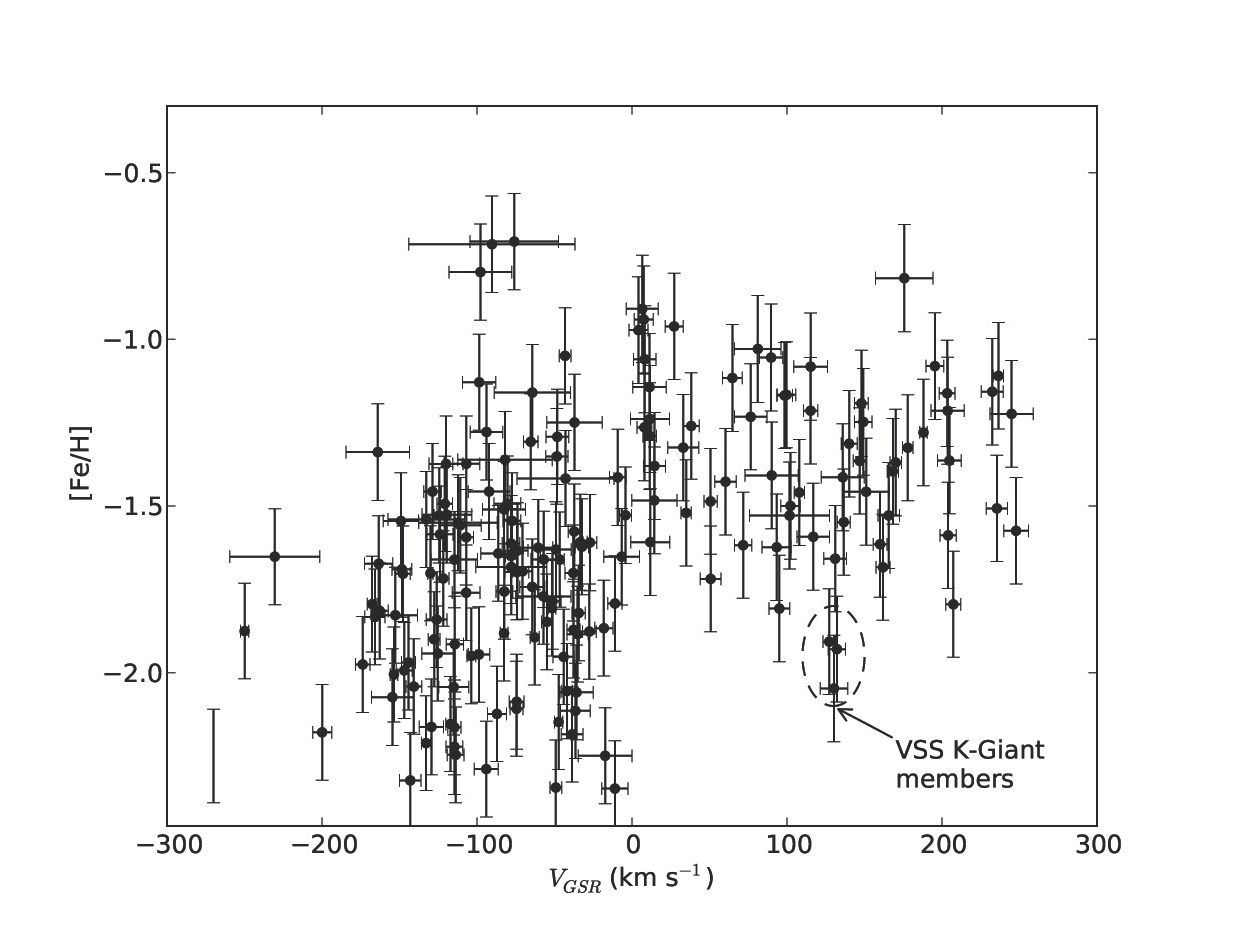
\includegraphics[width=9.2cm]{./figures/vss-candidates_copy.eps}
		\caption{Galactocentric velocities and metallicity measurements for K-giants in our sample. Highly likely VSS K-giant candidates are identified.}
		\label{fig:velocity-metallicity}
	\end{figure}
	
	The most likely VSS K-giant members are visibly separated from the bulk sample in velocity-metallicity space. Of the four candidates highlighted, three are highly probable VSS members, and another giant could be a member of VSS \--- given the error in metallicity. Galactocentric velocities of these candidates ranges from $V_{GSR} = 127$ to $132$ km s$^{-1}$; which matches the kinematic signature seen by others studying the VSS. Furthermore the metallicities of our most probable candidates range from [Fe/H] = -1.89 to -2.03, identical to metallicity measurements of the VSS found by \citet{Prior;et-al_2009a} using RR Lyraes. Although RR Lyraes are typically representative of an older, more metal-poor population, it is interesting that these candidates match the VSS characteristics in spatial position, velocity, and metallicity.

	High resolution follow-up spectroscopy on these targets will provide crucial information about the origin of the VSS. K-Giants are the perfect candidate for high resolution spectroscopy, as they are cool enough to provide detailed elemental abundances, from which the formation history of the parent origin can be inferred. Investigating [$\alpha$/Fe] ratios in these candidates can discern whether the origin of the VSS was a dSph \citep{Venn;et-al_2004, Casetti-Dinescu;et-al_2009}. Furthermore, high resolution spectroscopy will also help untangle (or perhaps strengthen) the relationship between the VSS and the VOD. Future observations are planned.

	\subsection{Carbon Stars}
		
		In our sample we have identified five carbon stars as contaminants. With the colour selections made to target K-giants, this region also overlaps with where we would expect to find carbon stars. Although these stars were not specifically targeted, their surface densities are so low \citep[$\approx$ 1 per 50 deg$^2$;][]{Green;et-al_1994} and our sky coverage is small ($\sim$ 8 deg$^2$), such that we would not expect them to be a large contaminant. All five carbon stars in are data are recognisable by the presence of distinctive 4737- and 5165 \AA\, Swan C$_2$ bands.
	
	\begin{figure}[h]
		\centering
		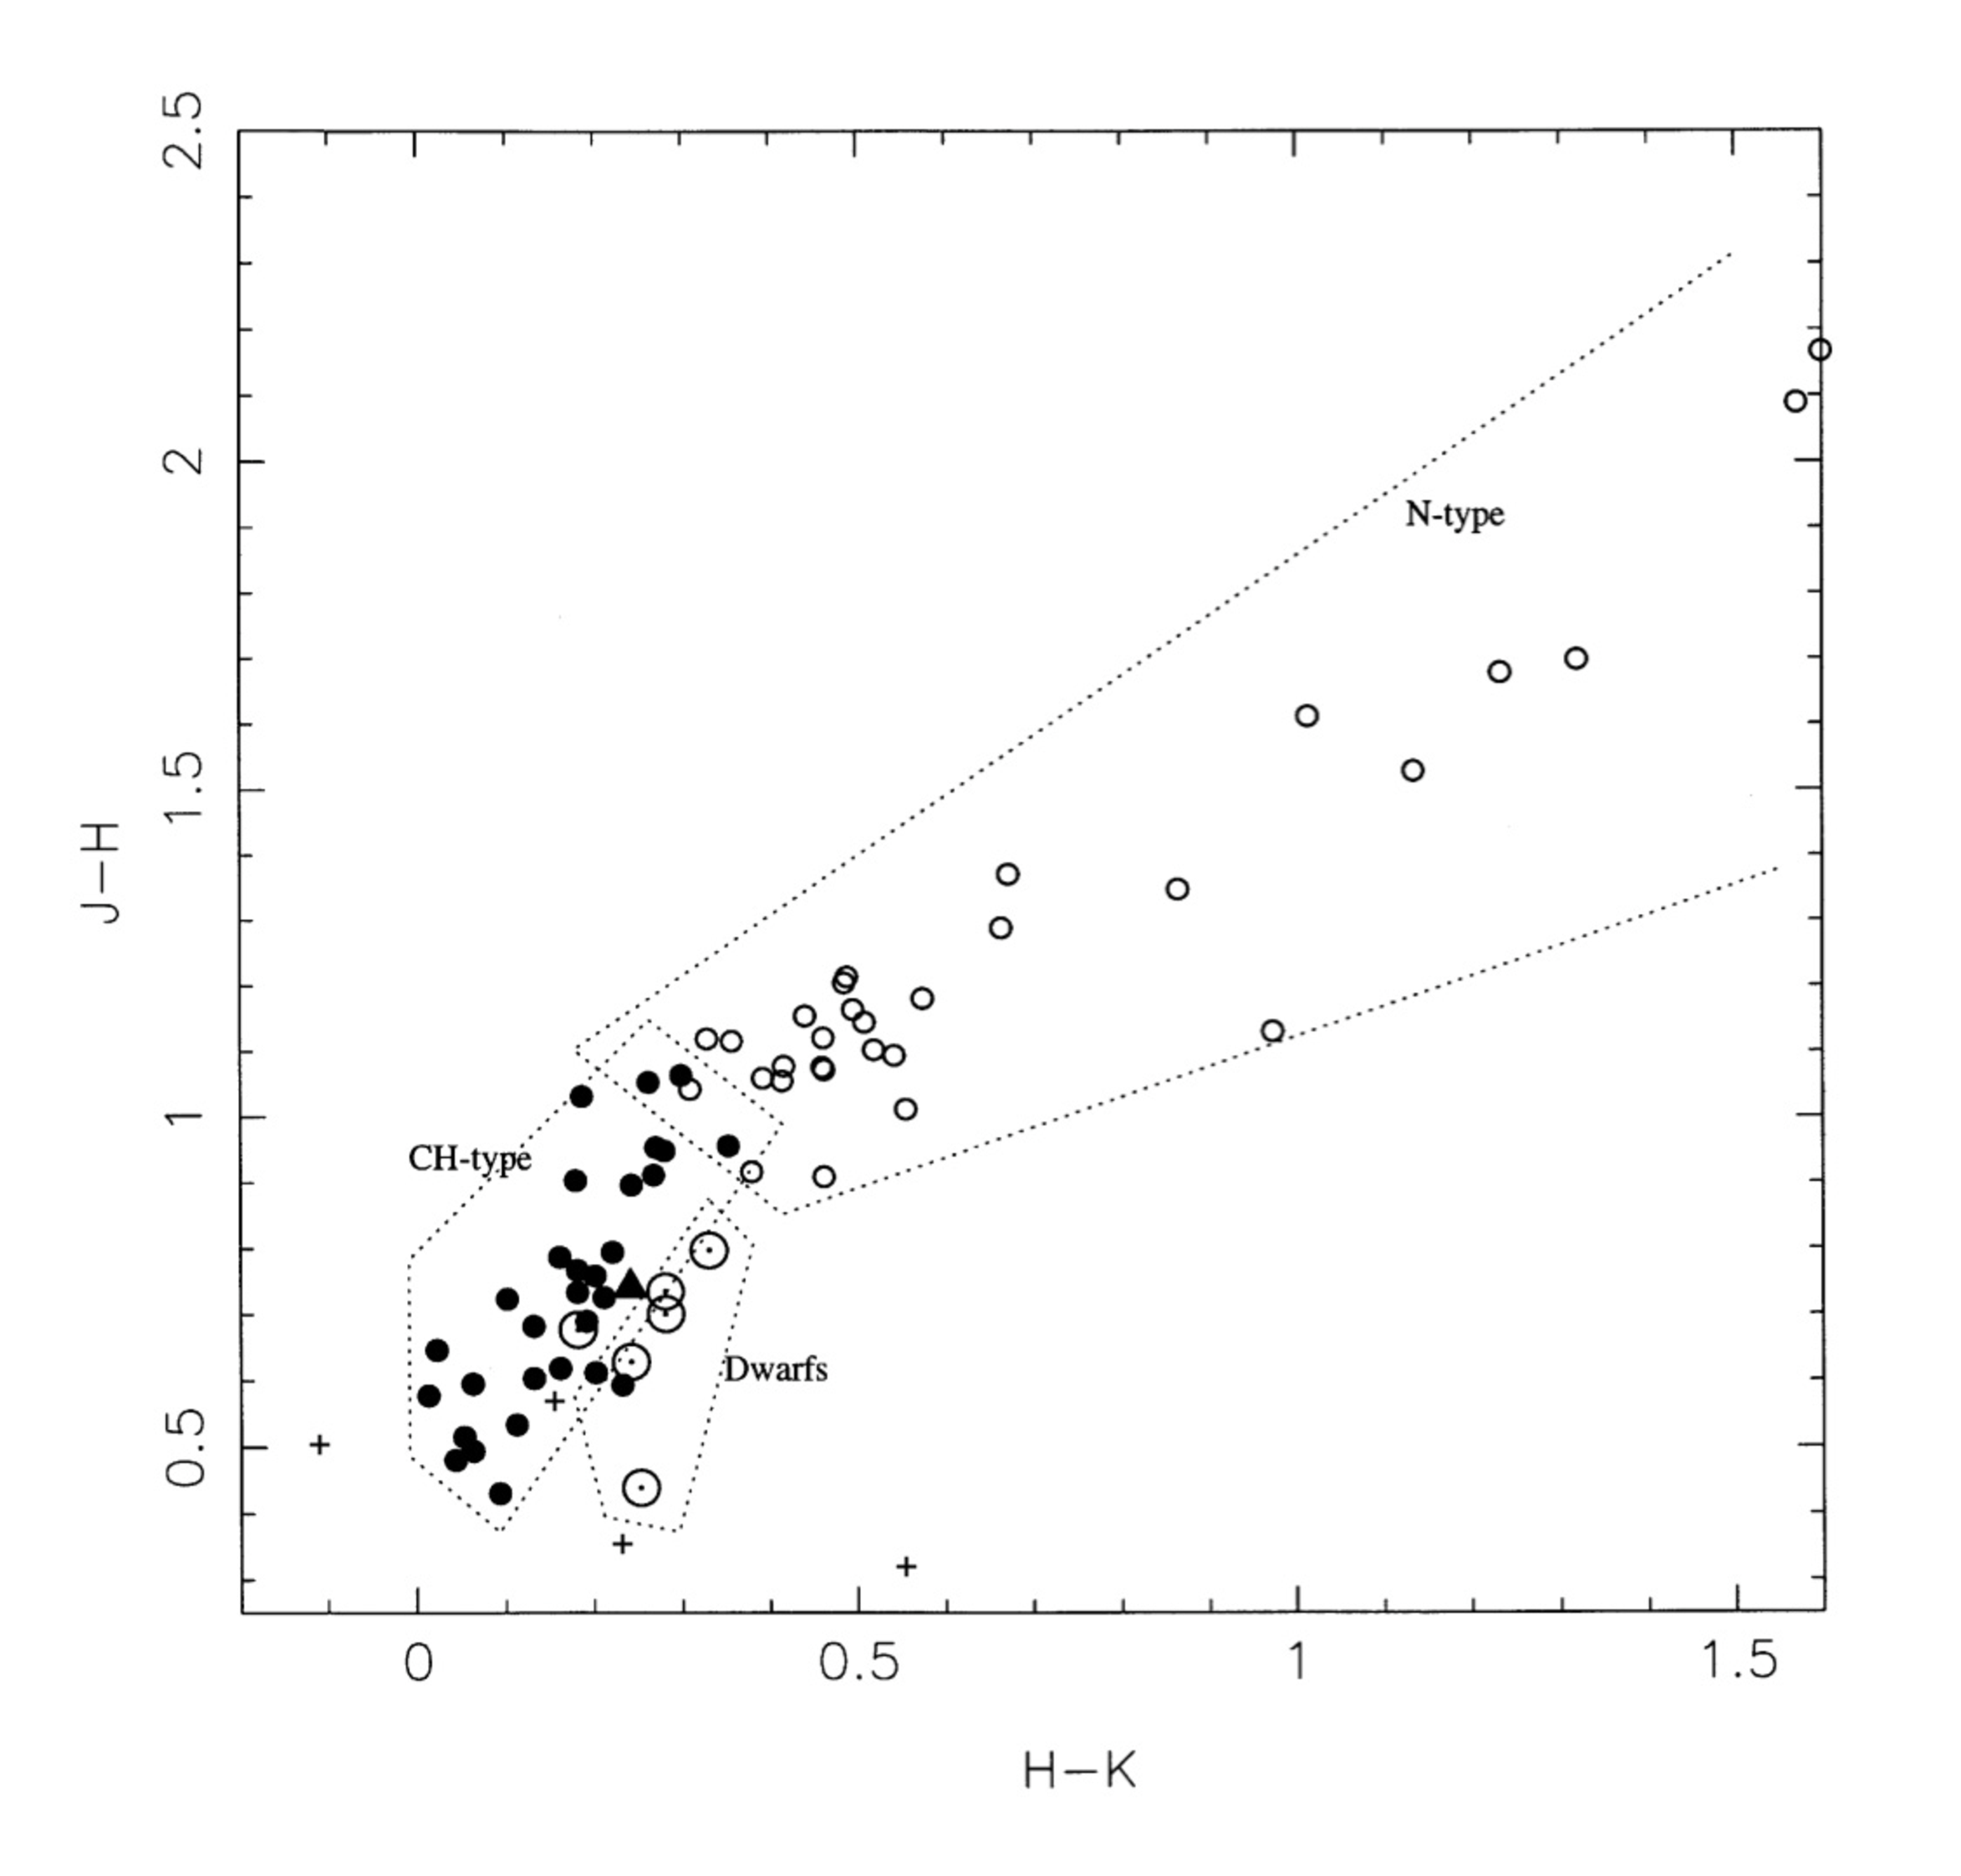
\includegraphics[width=9.1cm]{./figures/carbon.eps}
		\caption{J-H and H-K colours for carbon stars recovered by \citet{Totten;et-al_2000}, and those found in this sample. Four of our five carbon stars are represented with plus symbols (+); \textit{JHK} photometry for our faintest carbon star was not available. \\ This plot is an adaptation of Figure 3 in \citet{Totten;et-al_2000}}
		\label{fig:carbon-colours}
	\end{figure}
		
	There are at least three kinds of carbon stars present in the halo; (i) N-type carbon stars, (ii) giant CH-type carbon stars and (iii) and dwarf CH-type carbon stars \citep{Totten;Irwin_1998}. N-type carbon stars are formed by carbon-enriched dredge-up during the post-main-sequence phase of a normal asymptotic giant branch (AGB) star. First generation carbon stars (CH-type) are not considered to have undergone carbon-enriched dredge-up, and their carbon abundance is attributable to mass transfer within a binary system. Dwarf carbon stars emit a spectral signature which mimics that of a typical CH-type giant carbon star, however they have anomalous JHK colours \citep{Green;et-al_1992} and unusually high proper motions. These dwarf carbon stars are believed to form in binary systems where material has accreted from a now-invisible companion during its ascent up to the AGB \citep{Dahn;et-al_1977}.
	
	Giant CH-type carbon stars are similar to metal-poor carbon stars found in globular clusters \citep{Harding_1962} and in some dSph galaxies (\#citation needed) . The existence of the 4300 \AA\,CH g-band is representative of a CH-type carbon star, and is found in all five of our carbon stars. SDSS photometry for our stars match well with the F/G-type CH carbon stars identified by \citet{Downes;et-al_2004}.The JHK colours of our entire carbon sample are characteristic of the F/G-type CH carbon stars found by \citet{Totten;Irwin_1998} in their cool carbon star survey (Figure \ref{fig:carbon-colours}). None of our stars exhibit significant proper motion, which strongly suggests they are not dwarfs \citep{Green;et-al_1994, Deutsch_1994}. 


\begin{figure}[h]
	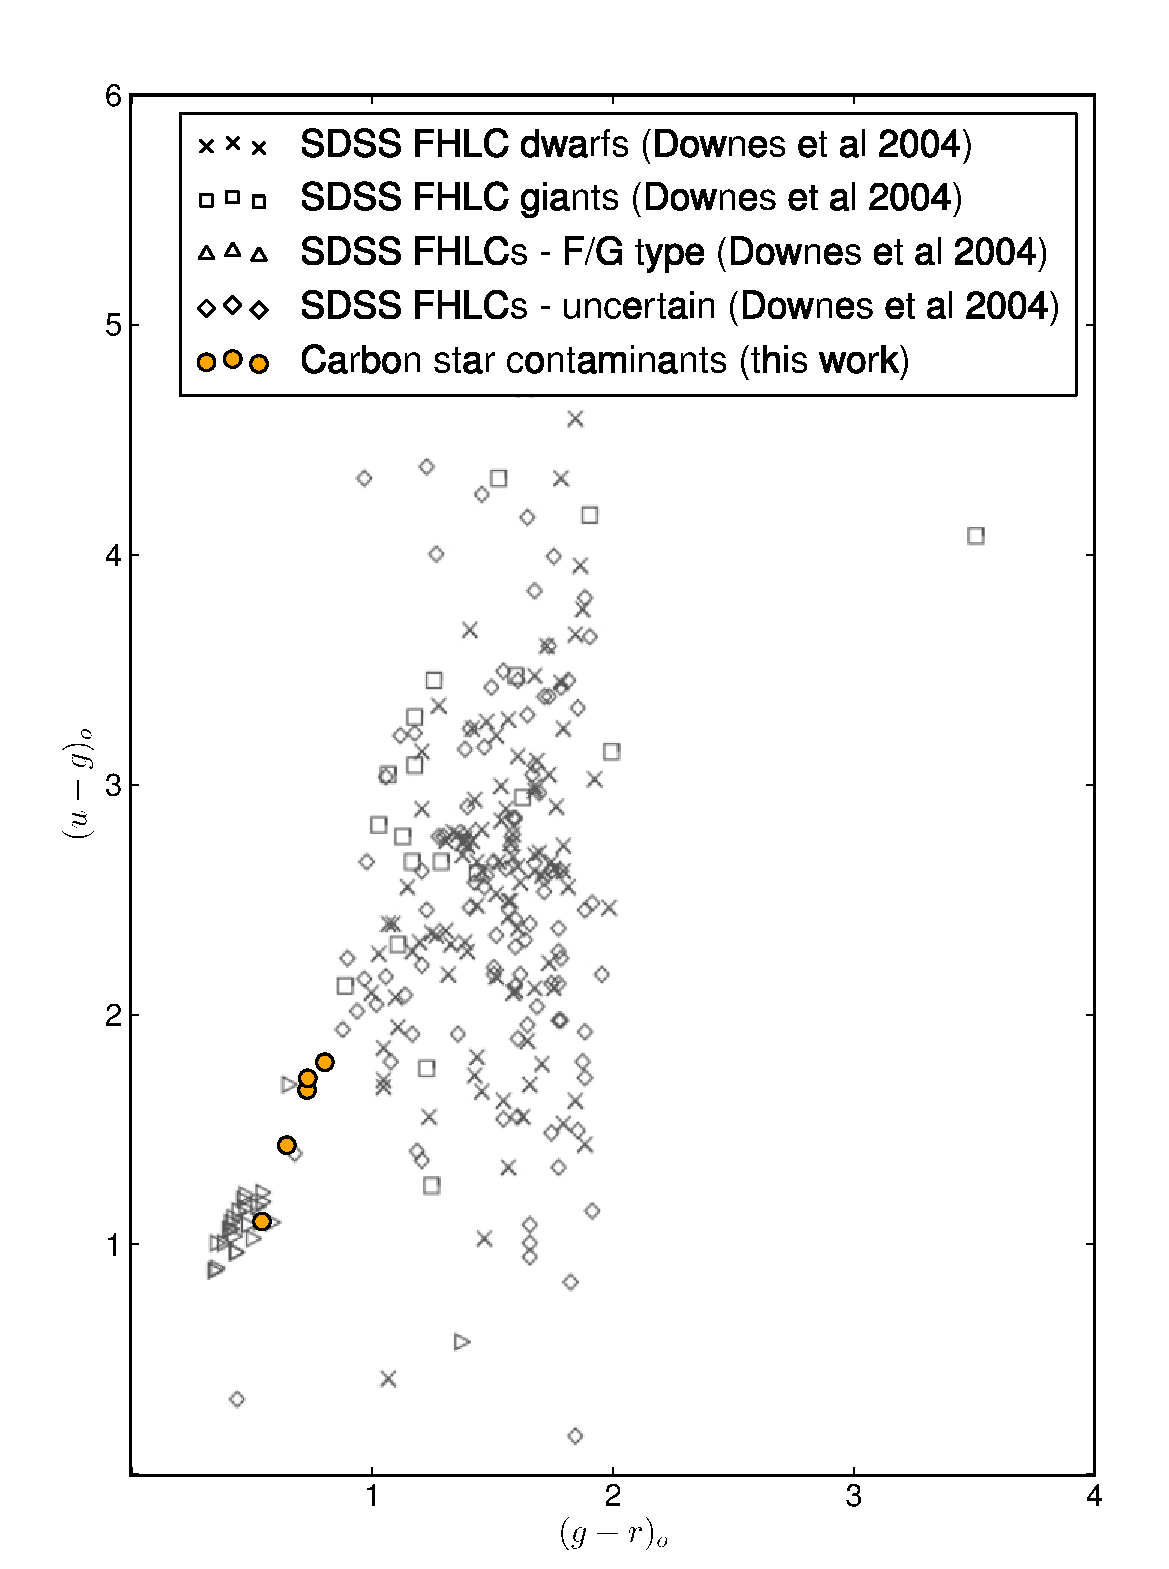
\includegraphics[width=9.2cm]{./figures/carbonstarcolor.eps}
	\caption{Sloan \textit{u \-- g} and \textit{g \--- r} colours for our carbon stars, and the identified carbon star populations from SDSS.}
	\label{fig:carbon-sdss}
\end{figure}

	\begin{table*}[t]
	\centering
	{\hfill{}
		\begin{tabular}{c c c c c c c c c c}
		\toprule
		\multirow{2}{*}{SDSS Name J+\tablenotemark{a}}	&\multirow{2}{*}{\textit{u-g}}	& \multirow{2}{*}{\textit{g-r}}	& \multirow{2}{*}{\textit{r-i}} & \multirow{2}{*}{\textit{i-z}} & \multirow{2}{*}{\textit{J-H}} & \multirow{2}{*}{\textit{H-K}} & $\mu$ & $V_{GSR}$		& [Fe/H]	\\
									&		 	&		  	&			&			&			& &	(mas yr$^{-1}$)       	&(km s$^{-1}$)		& (dex)	\\ 
		\toprule
		121740.94-001839.5				& 1.10		& 0.54		& 0.16 		& 0.05		& ...\tablenotemark{b}& ...\tablenotemark{b}	& $15.0 \pm 4.2$ & $\:-59 \pm 33\;$	& $-1.78 \pm 0.16$ \\
		121853.18-004628.4				& 1.67		& 0.73 		& 0.22		& 0.11		& 0.36		& 0.24		& $\:\:3.2 \pm 4.2$ & $\:-31 \pm 8.5$	& $-0.87 \pm 0.16$ \\
		122053.71-011709.5  				& 1.79		& 0.80		& 0.26		& 0.13		& 0.56		& 0.16		& $\:\:2.8 \pm 4.2$ & $\:+25 \pm 3.9$	& $-1.23 \pm 0.16$ \\
		125410.80-032744.0				& 1.43		& 0.64		& 0.22		& 0.05		& 0.32		& 0.56		& $18.8 \pm 4.2$ & $\:+40 \pm 9.9$	& $-1.24 \pm 0.16$ \\	
		125416.52-031437.6				& 1.72		& 0.73		& 0.25		& 0.11		& 0.50		& -0.11\:	 	& $15.5 \pm 4.2$ & $+182 \pm 8.2\;$	& $-1.60 \pm 0.16$ \\
		
		\bottomrule
		\end{tabular}
		
	
	}
	\hfill{}
	\caption{Object names and measurements for the five F/G-type CH carbon stars found within our sample.}
	\label{tb:carbon-stars}
	%\tablenotetext{a}{In keeping with convention, positional information has been truncated. Full information is available through the SDSS archive.}
	%\tablenotetext{b}{No \textit{JHK} photometry is available for this object as it is fainter than the 2MASS limit.}

	\end{table*}
	

	As these stars were selected from the SDSS catalogue, \textit{ugriz} photometry is available. However they were not spectroscopically observed in the follow-up SEGUE survey. Through comparisons with previous carbon-type star catalogues \citep{Totten;Irwin_1998, Downes;et-al_2004, Goswami;et-al_2010}, the stars tabulated in Table \ref{tb:carbon-stars} are previously unclassified. This is largely because our stars are too faint to have been classified by previous carbon surveys. The kinematics of our carbon stars are representative of a typical halo population.


	
	\section{Conclusions}
	\label{sec:conclusions}
	
	Lorem ipsum dolor sit amet, consectetur adipiscing elit. Vestibulum malesuada placerat tellus et hendrerit. Praesent eu velit vel velit suscipit scelerisque. Vestibulum pellentesque suscipit felis. Proin et ligula euismod lectus convallis ornare vitae ut diam. Aliquam scelerisque vehicula porta. Integer vulputate vulputate tempor. Mauris tincidunt nunc ac magna tincidunt dapibus. Nam auctor suscipit sapien, sed vestibulum enim lacinia vel. Fusce ullamcorper volutpat vehicula. Phasellus ornare rutrum facilisis. In tristique scelerisque nisl vitae ornare. Etiam varius consectetur sapien, sed lobortis mauris interdum ac. Integer leo urna, sodales in venenatis eu, ultrices ut nunc. Donec vestibulum dui et sem ultricies vel posuere ligula iaculis. Etiam gravida gravida augue non congue. Quisque lorem eros, faucibus non lacinia sit amet, imperdiet id metus.
	
	Lorem ipsum dolor sit amet, cosectetur adipiscing elit. Vestibulum malesuada placerat tellus et hendrerit. Praesent eu velit vel velit suscipit scelerisque. Vestibulum pellentesque suscipit felis. Proin et ligula euismod lectus convallis ornare vitae ut diam. Aliquam scelerisque vehicula porta. Integer vulputate vulputate tempor. Mauris tincidunt nunc ac magna tincidunt dapibus. Nam auctor suscipit sapien, sed vestibulum enim lacinia vel. Fusce ullamcorper volutpat vehicula. Phasellus ornare rutrum facilisis. In tristique scelerisque nisl vitae ornare. Etiam varius consectetur sapien, sed lobortis mauris interdum ac. Integer leo urna, sodales in venenatis eu, ultrices ut nunc. Donec vestibulum dui et sem ultricies vel posuere ligula iaculis. Etiam gravida gravida augue non congue. 
	
\bibliographystyle{hapj}
\bibliography{draft}

\end{document}